\newpage
\chapter{Application Development}
\label{chap:frontend}

In this chapter, we will focus on the frontend development of our money management application. We will discuss the technologies and tools used, the implementation of the user interface, and the enhancements made to improve the user experience.

\section{Technologies and Tools}
\label{sec:frontend-tech}
 \subsection{Technologies}
In this paper, the following technologies have been employed for development:



\begin{itemize}
\item \textbf{React Native}: React Native is a TypeScript framework used for building mobile applications. It allows developers to create native-like apps for iOS and Android platforms using a single codebase. React Native leverages the power of TypeScript and React to deliver high-performance and visually appealing mobile applications \cite{reactnative}.

\item \textbf{Expo}: Expo is a set of tools and services built around React Native that simplifies the development process. It provides an integrated development environment (IDE) and various libraries to streamline the frontend development workflow. Expo offers features such as hot reloading, over-the-air updates, and built-in APIs that enhance productivity and app functionality \cite{expo}.

\item \textbf{TypeScript}: TypeScript is a statically typed superset of JavaScript that brings additional features and benefits to the development process. It introduces static typing, enabling developers to catch potential errors and bugs early in the development phase. TypeScript enhances code readability, provides better tooling support, and improves the overall maintainability of the codebase \cite{typescript}.

\item \textbf{GraphQL}: GraphQL is a query language for APIs and a runtime for executing queries with existing data. It allows clients to specify the data they need, and the server responds with only the requested data, reducing over-fetching and under-fetching of data. GraphQL simplifies data fetching and manipulation, improves performance, and provides a flexible and efficient approach to API development \cite{graphql}.
\end{itemize}


By utilizing React Native, Expo, TypeScript, and GraphQL, this paper's development ensures efficient cross-platform app development, simplified workflow, enhanced productivity, improved code quality, and effective data handling. These technologies work together to deliver a robust and user-friendly mobile application experience.

\subsection{Tools}
In the frontend development process, the following tools have been utilized:

\begin{itemize}
\item \textbf{Figma}: Figma is a cloud-based design and prototyping tool that enables collaborative interface design. It provides a user-friendly interface for creating and sharing design mockups, wireframes, and interactive prototypes. Figma allows designers and developers to collaborate in real time, making it easier to iterate on the design and ensure a cohesive user experience \cite{figma}.

\item \textbf{WebStorm}: WebStorm is an integrated development environment (IDE) specifically designed for web development. It offers a wide range of features, including intelligent code completion, code analysis, and debugging capabilities. WebStorm provides a smooth development experience for writing and managing TypeScript, JavaScript, HTML, and CSS code, making it an ideal choice for frontend development. \cite{webstorm}

\item \textbf{Expo Go}: Expo Go is a mobile app that enables developers to test and preview their React Native applications in real-time on physical devices. It allows developers to quickly iterate and view changes made to the app without the need for complicated setup or app building processes. Expo Go provides a convenient way to test app functionality and UI responsiveness during the development phase \cite{expogo}.

\item \textbf{React Developer Tools}: React Developer Tools is a browser extension that enhances the development experience for React applications. It provides a set of debugging and inspection tools specifically tailored for React components. Developers can inspect component hierarchies, view state and props, and track component updates in real-time. React Developer Tools greatly aids in understanding and troubleshooting React components during frontend development \cite{reactdevtools}.

\item \textbf{Apollo Studio}: Apollo Studio is a powerful tool for managing, monitoring, and analyzing GraphQL APIs. It provides a comprehensive platform that enables developers to design, document, and collaborate on GraphQL schemas, track API usage, and gain insights into performance and errors. With Apollo Studio, developers can easily optimize their GraphQL APIs, debug issues, and ensure efficient data delivery to frontend applications. It offers features such as schema management, query performance tracking, error tracking, and integration with popular development tools. By incorporating Apollo Studio into the frontend development process, developers can enhance the overall GraphQL API development experience and deliver high-quality and performant applications \cite{apollostudio}.

\end{itemize}


These tools enhance the frontend development process, enabling developers to streamline their workflow, ensure code quality, and deliver high-quality mobile applications. Each tool plays a unique role in supporting different aspects of frontend development, from design and coding to testing and monitoring. By leveraging these tools, developers can effectively collaborate, debug applications, perform real-time testing, optimize GraphQL APIs, and maintain code quality throughout the development lifecycle.



    \section{User Experience}
\label{sec:ux-enhancements}



In the context of app development, user flow refers to the series of steps a user takes while navigating through an application or interacting with its features. It encompasses the paths, actions, and interactions that users follow to accomplish their goals within the app.

User flow plays a crucial role in creating a seamless and intuitive user experience. By understanding and designing effective user flows, developers can guide users through the app's functionalities, ensuring they can easily access the desired information or perform specific actions.

In this section, the user flow of the application will be explored and analyzed, focusing on the key screens and interactions that users encounter during their journey. By examining the user flow, potential bottlenecks can be identified, usability can be improved, and the overall user experience can be optimized.
\newpage 
\subsection{User Flow: Transaction}

The registration process allows users to create an account and gain access to the application's features. It involves the following steps:

\begin{enumerate}
  \item User Arrival: The user arrives at the registration screen and is presented with a registration form.
  \item Input Fields: The registration form includes fields for name, email, password, and any additional required information.
  \item Validation: The user's input is validated to ensure accuracy and completeness. Error messages are displayed for any missing or invalid information.
  \item Create Account: Once all required information is provided, the user can proceed to create their account by clicking the "Create Account" button.
  \item Confirmation: A confirmation message is displayed to notify the user that their account has been successfully created.
\end{enumerate}


\begin{figure}[ht]
  \centering
  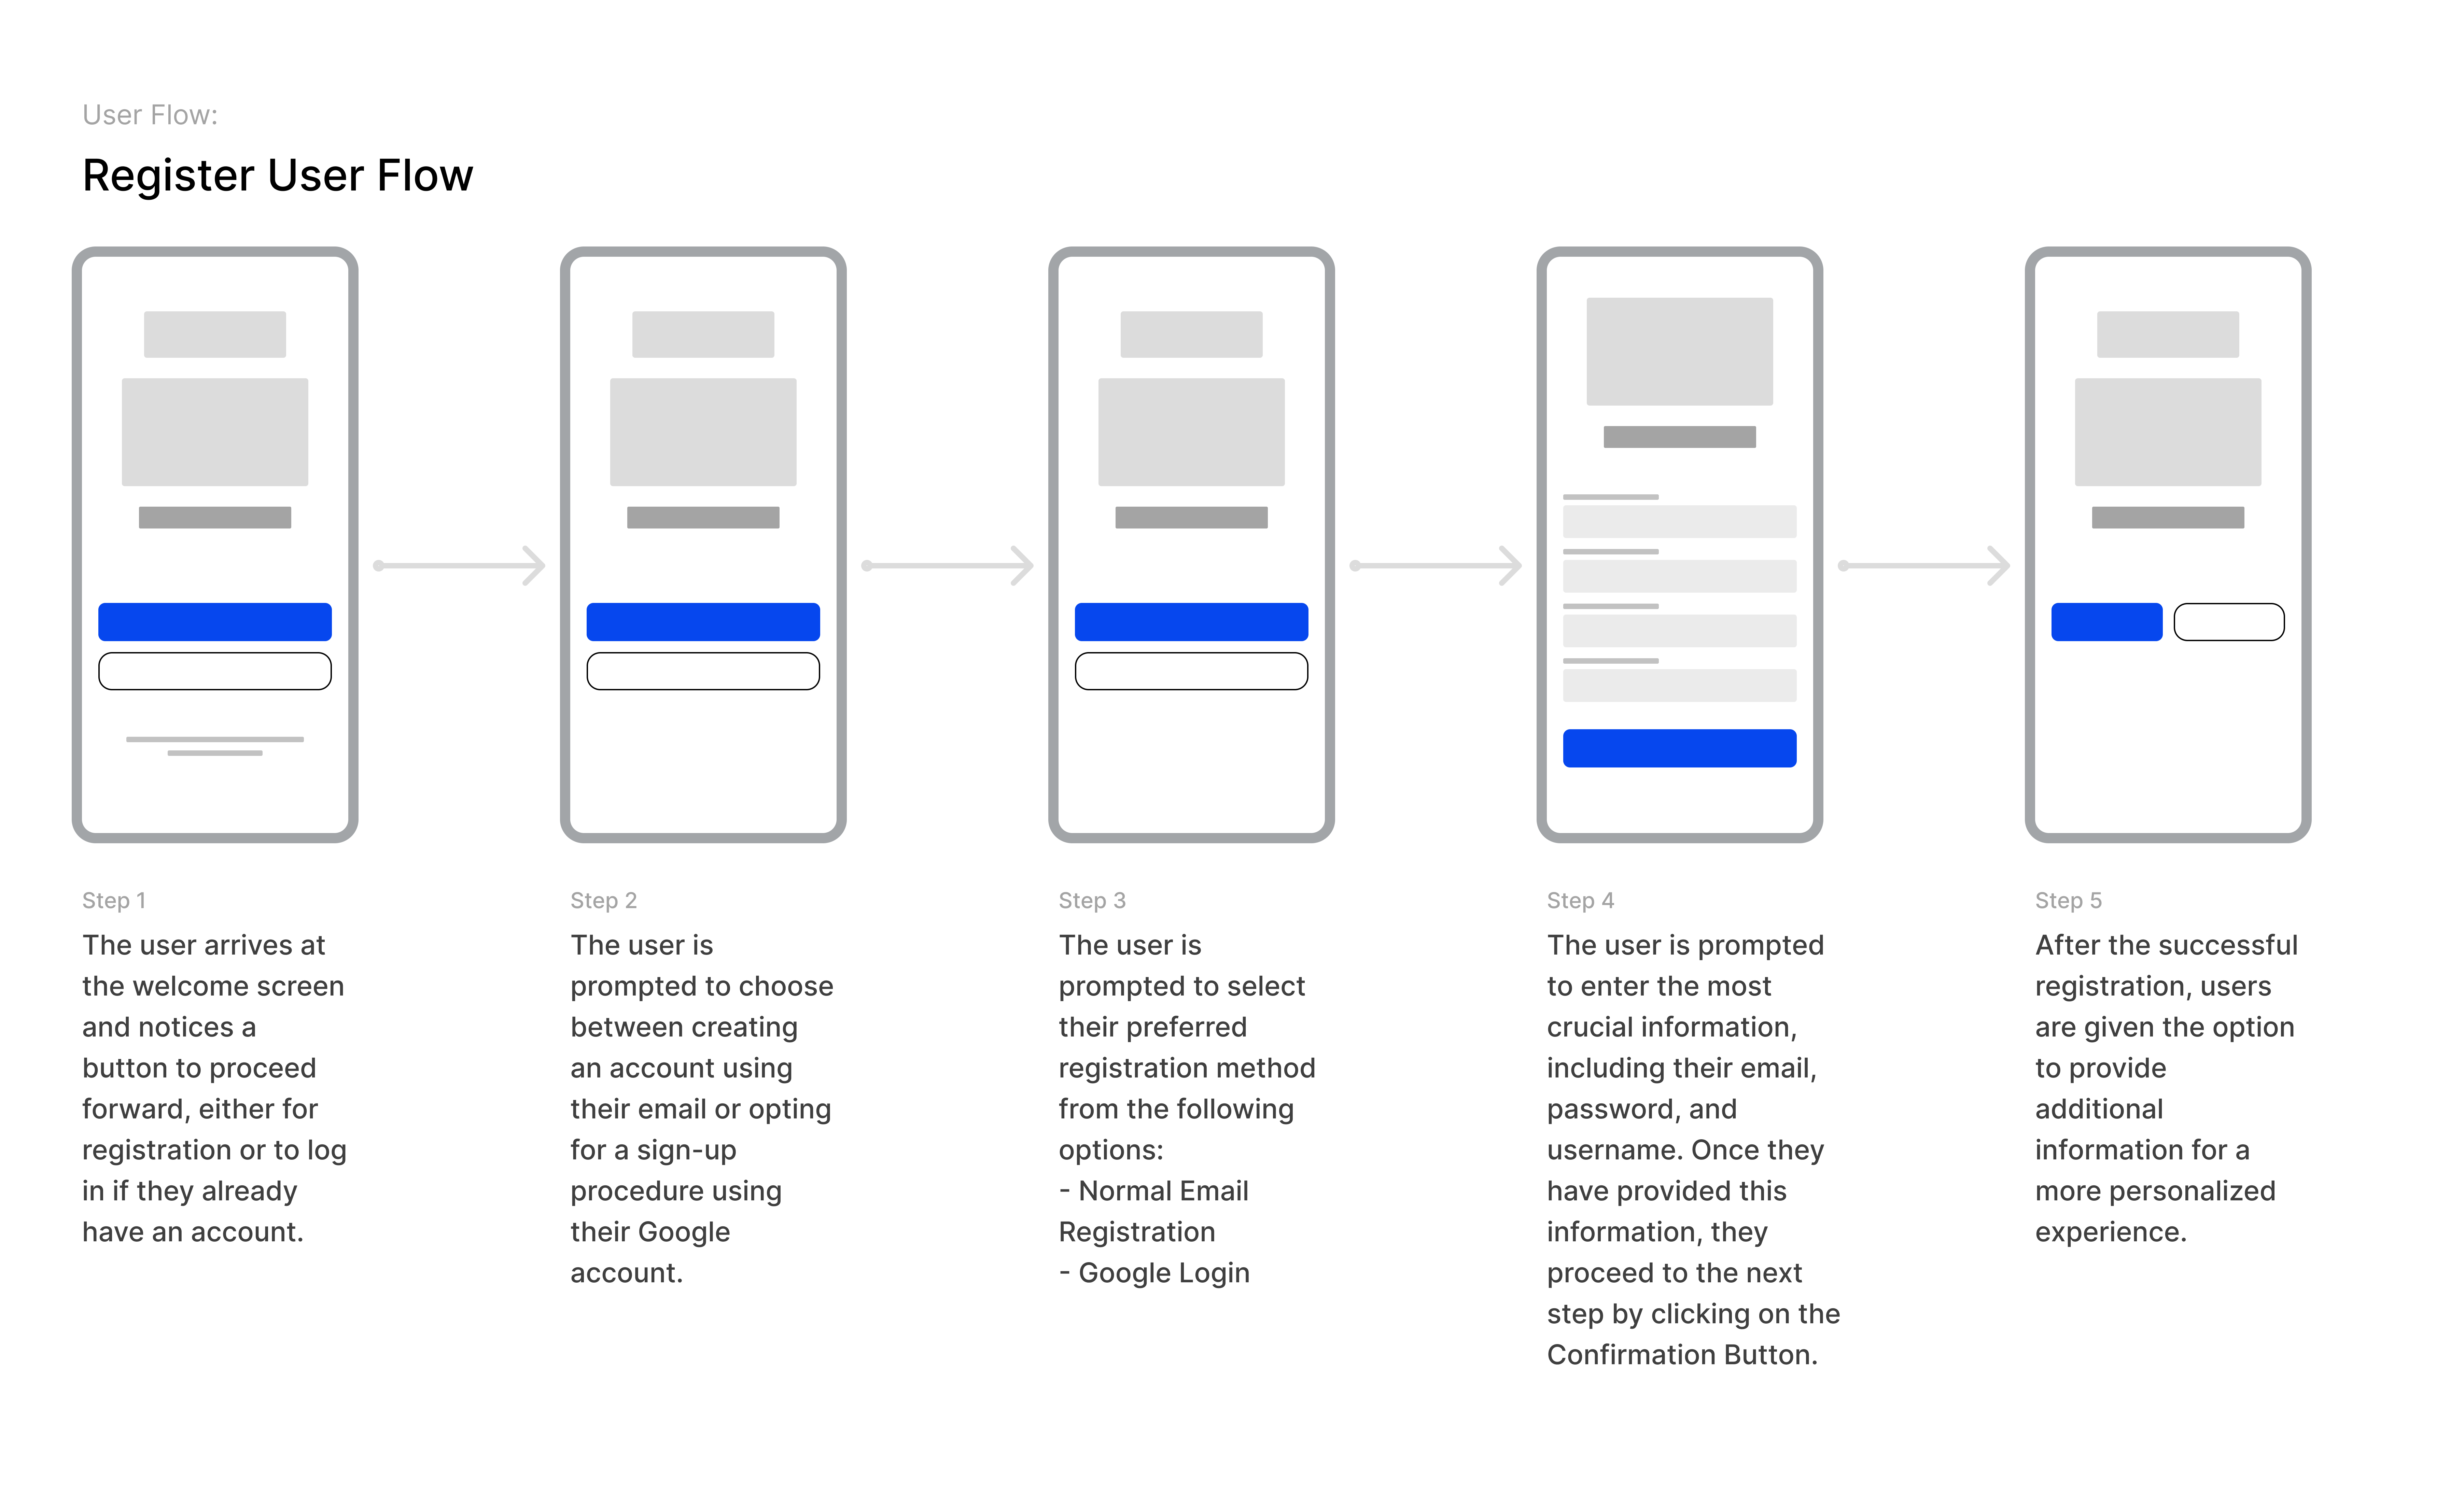
\includegraphics[width=\textwidth]{Graphics/UserFlows/RegisterUserFlow.png}
  \caption{User Flow: Registration Process}
  \label{fig:registration_flow}
\end{figure}

In Figure \ref{fig:registration_flow}, the image illustrates the sequential steps involved in the registration process, guiding the user from arrival to account creation.

This user flow prompt provides an overview of the registration process and complements the visual representation in the accompanying image.
\newpage
\subsection{User Flow: Login}

The login process allows registered users to access their accounts and utilize the application's features. It involves the following steps:

\begin{enumerate}
  \item User Arrival: The user arrives at the login screen and is presented with a login form.
  \item Input Fields: The login form includes fields for email and password.
  \item Validation: The user's input is validated to ensure accuracy and completeness. Error messages are displayed for any missing or incorrect information.
  \item Login: Once the user enters the correct email and password, they can proceed to login by clicking the "Login" button.
  \item Authentication: The user's credentials are authenticated against the stored account information.
  \item Redirect: Upon successful login, the user is redirected to the main page/dashboard of the application.
\end{enumerate}



\begin{figure}[ht]
  \centering
  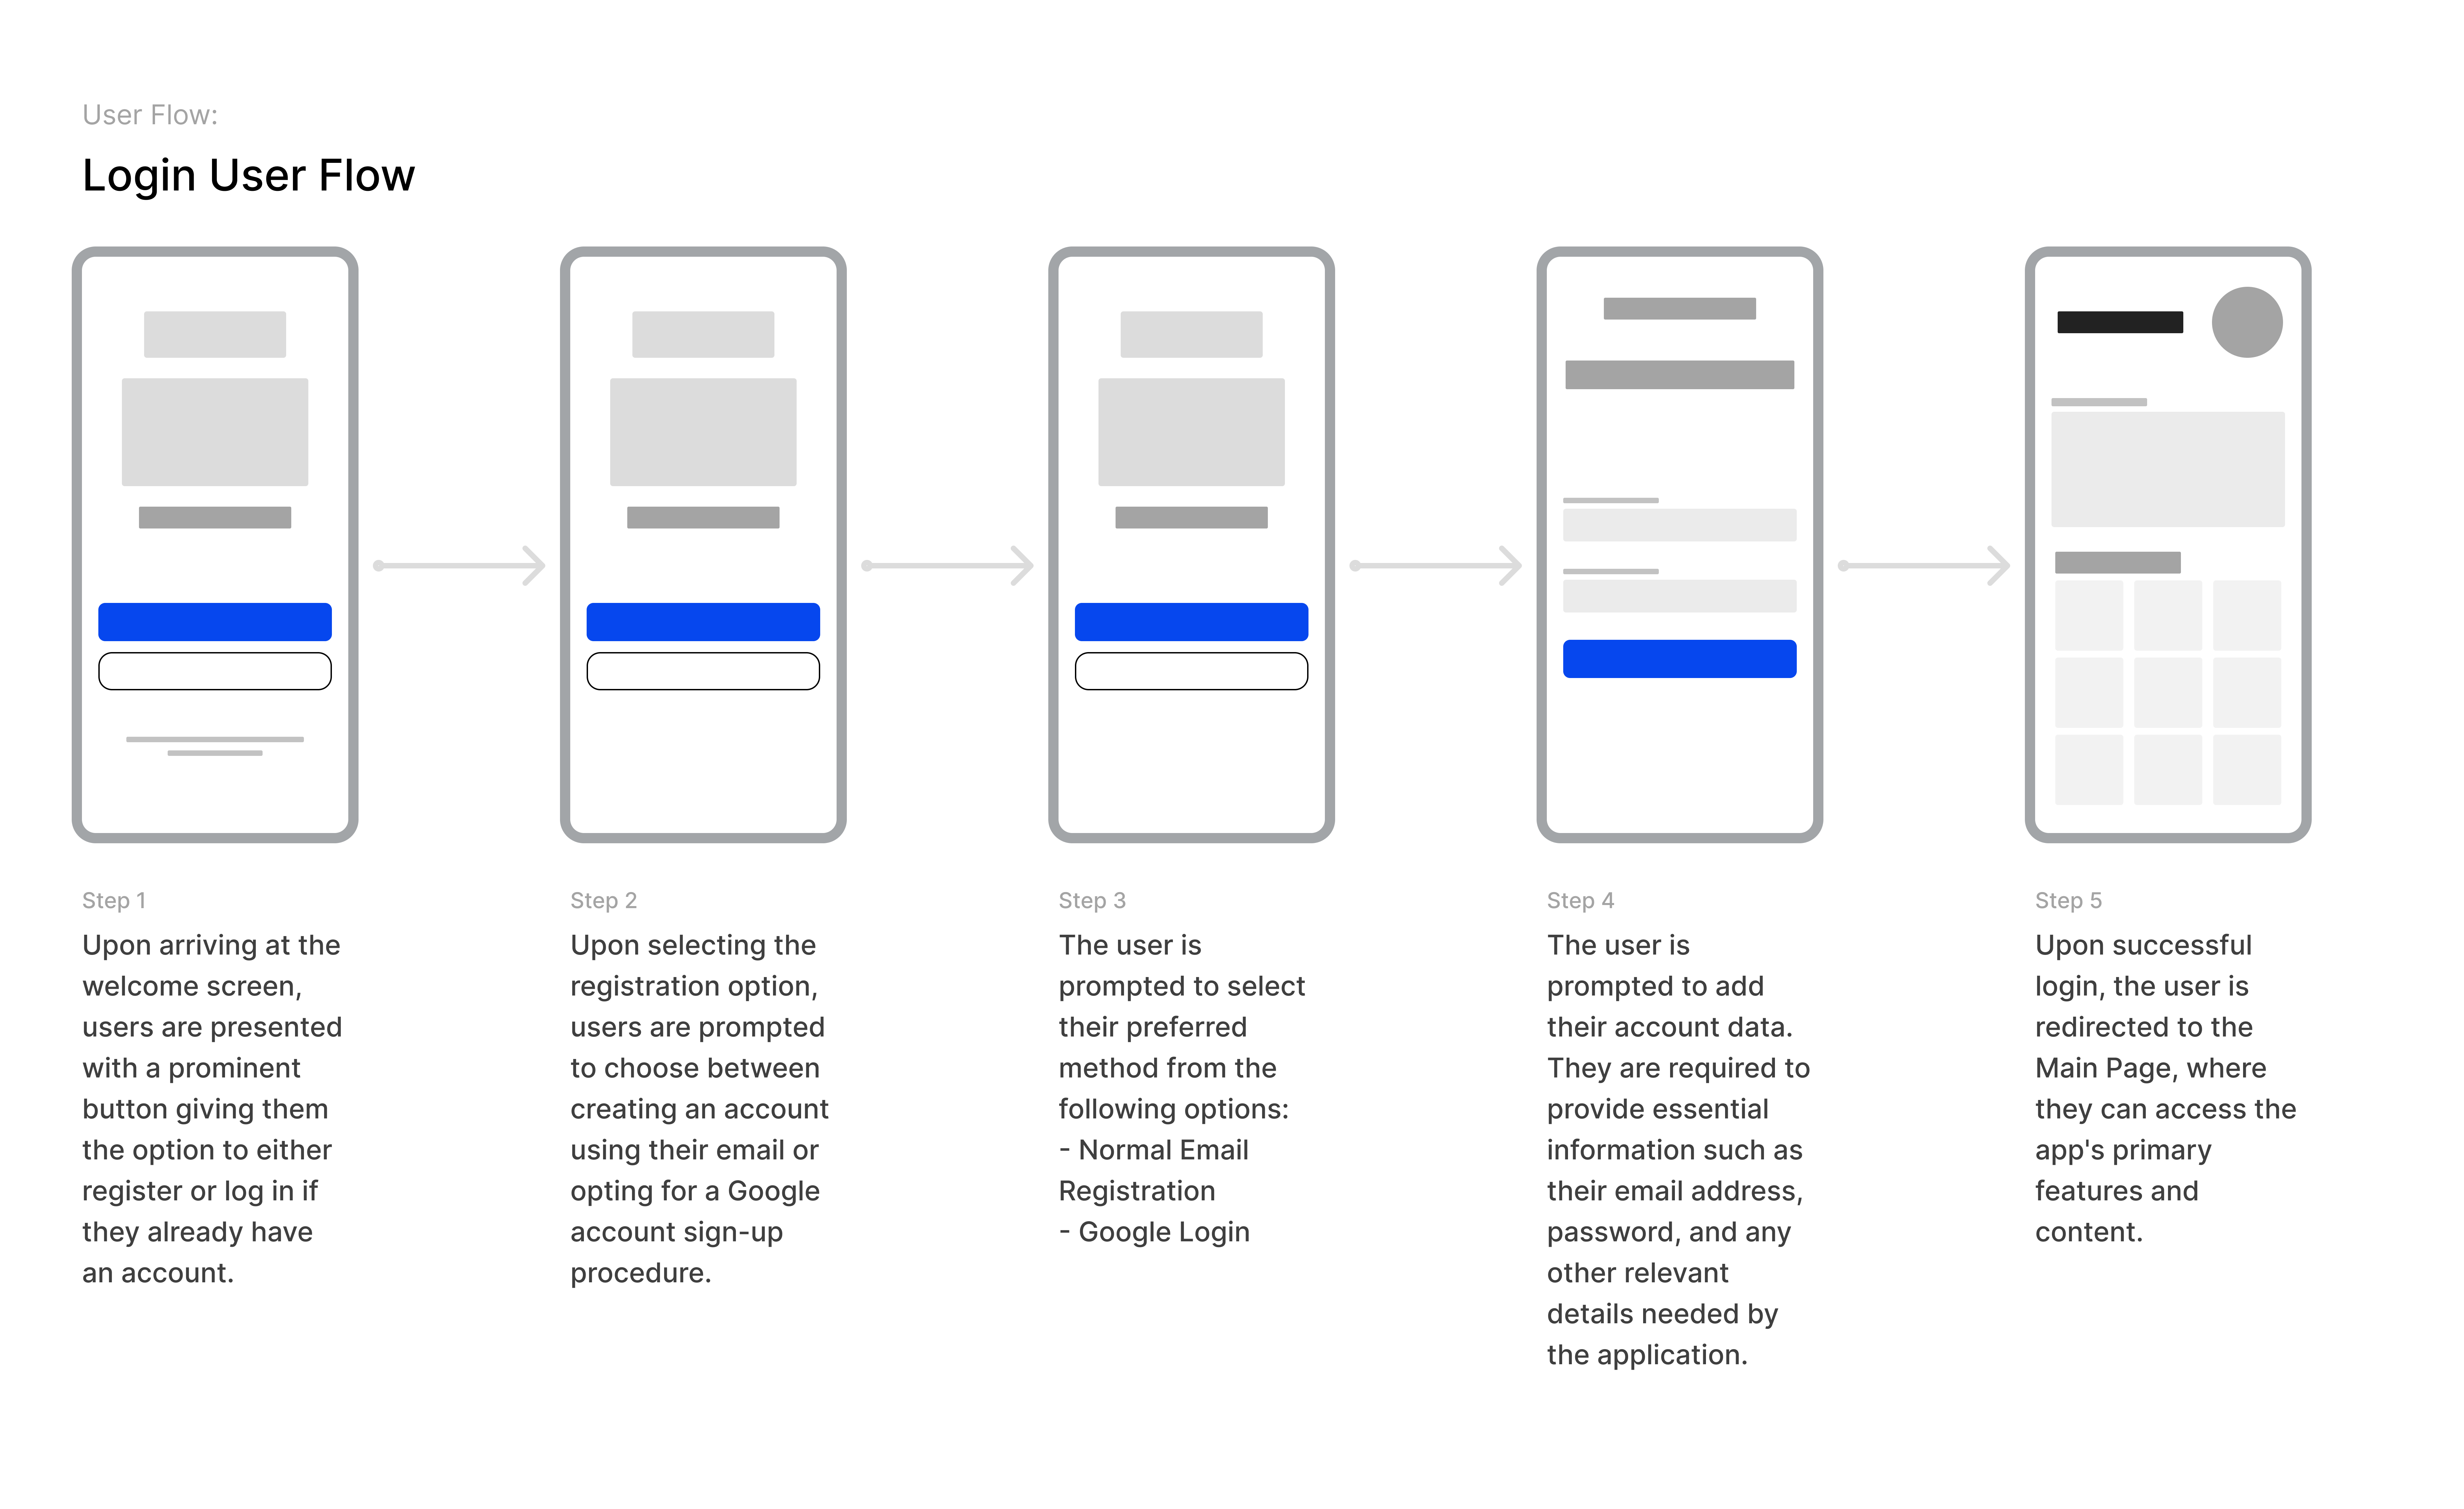
\includegraphics[width=\textwidth]{Graphics/UserFlows/LoginUserFlow.png}
  \caption{User Flow: Login Process}
  \label{fig:login_flow}
\end{figure}

In Figure \ref{fig:login_flow}, the image illustrates the sequential steps involved in the login process, guiding the user from arrival to successful authentication.

This user flow prompt provides an overview of the login process and complements the visual representation in the accompanying image.


\subsection{User flow: Transaction}

A transaction is a key interaction in the application where users can perform financial operations such as recording expenses or income. Let's explore the user flow for a typical transaction:


  \textbf{Step 1:} The user navigates to the transaction section of the app.
  
   \textbf{Step 2:} The user is presented with a form to enter transaction details, including the transaction type (expense or income), amount, category, and additional notes.
  
  \textbf{Step 3:} After filling in the required information, the user clicks on the "Submit" button to proceed.
  
   \textbf{Step 4:} The app validates the transaction data and performs any necessary calculations or checks.
  
   \textbf{Step 5:} If the transaction is successful, the app displays a confirmation message or animation to indicate that the transaction has been recorded.


\begin{figure}[h!]
  \centering
  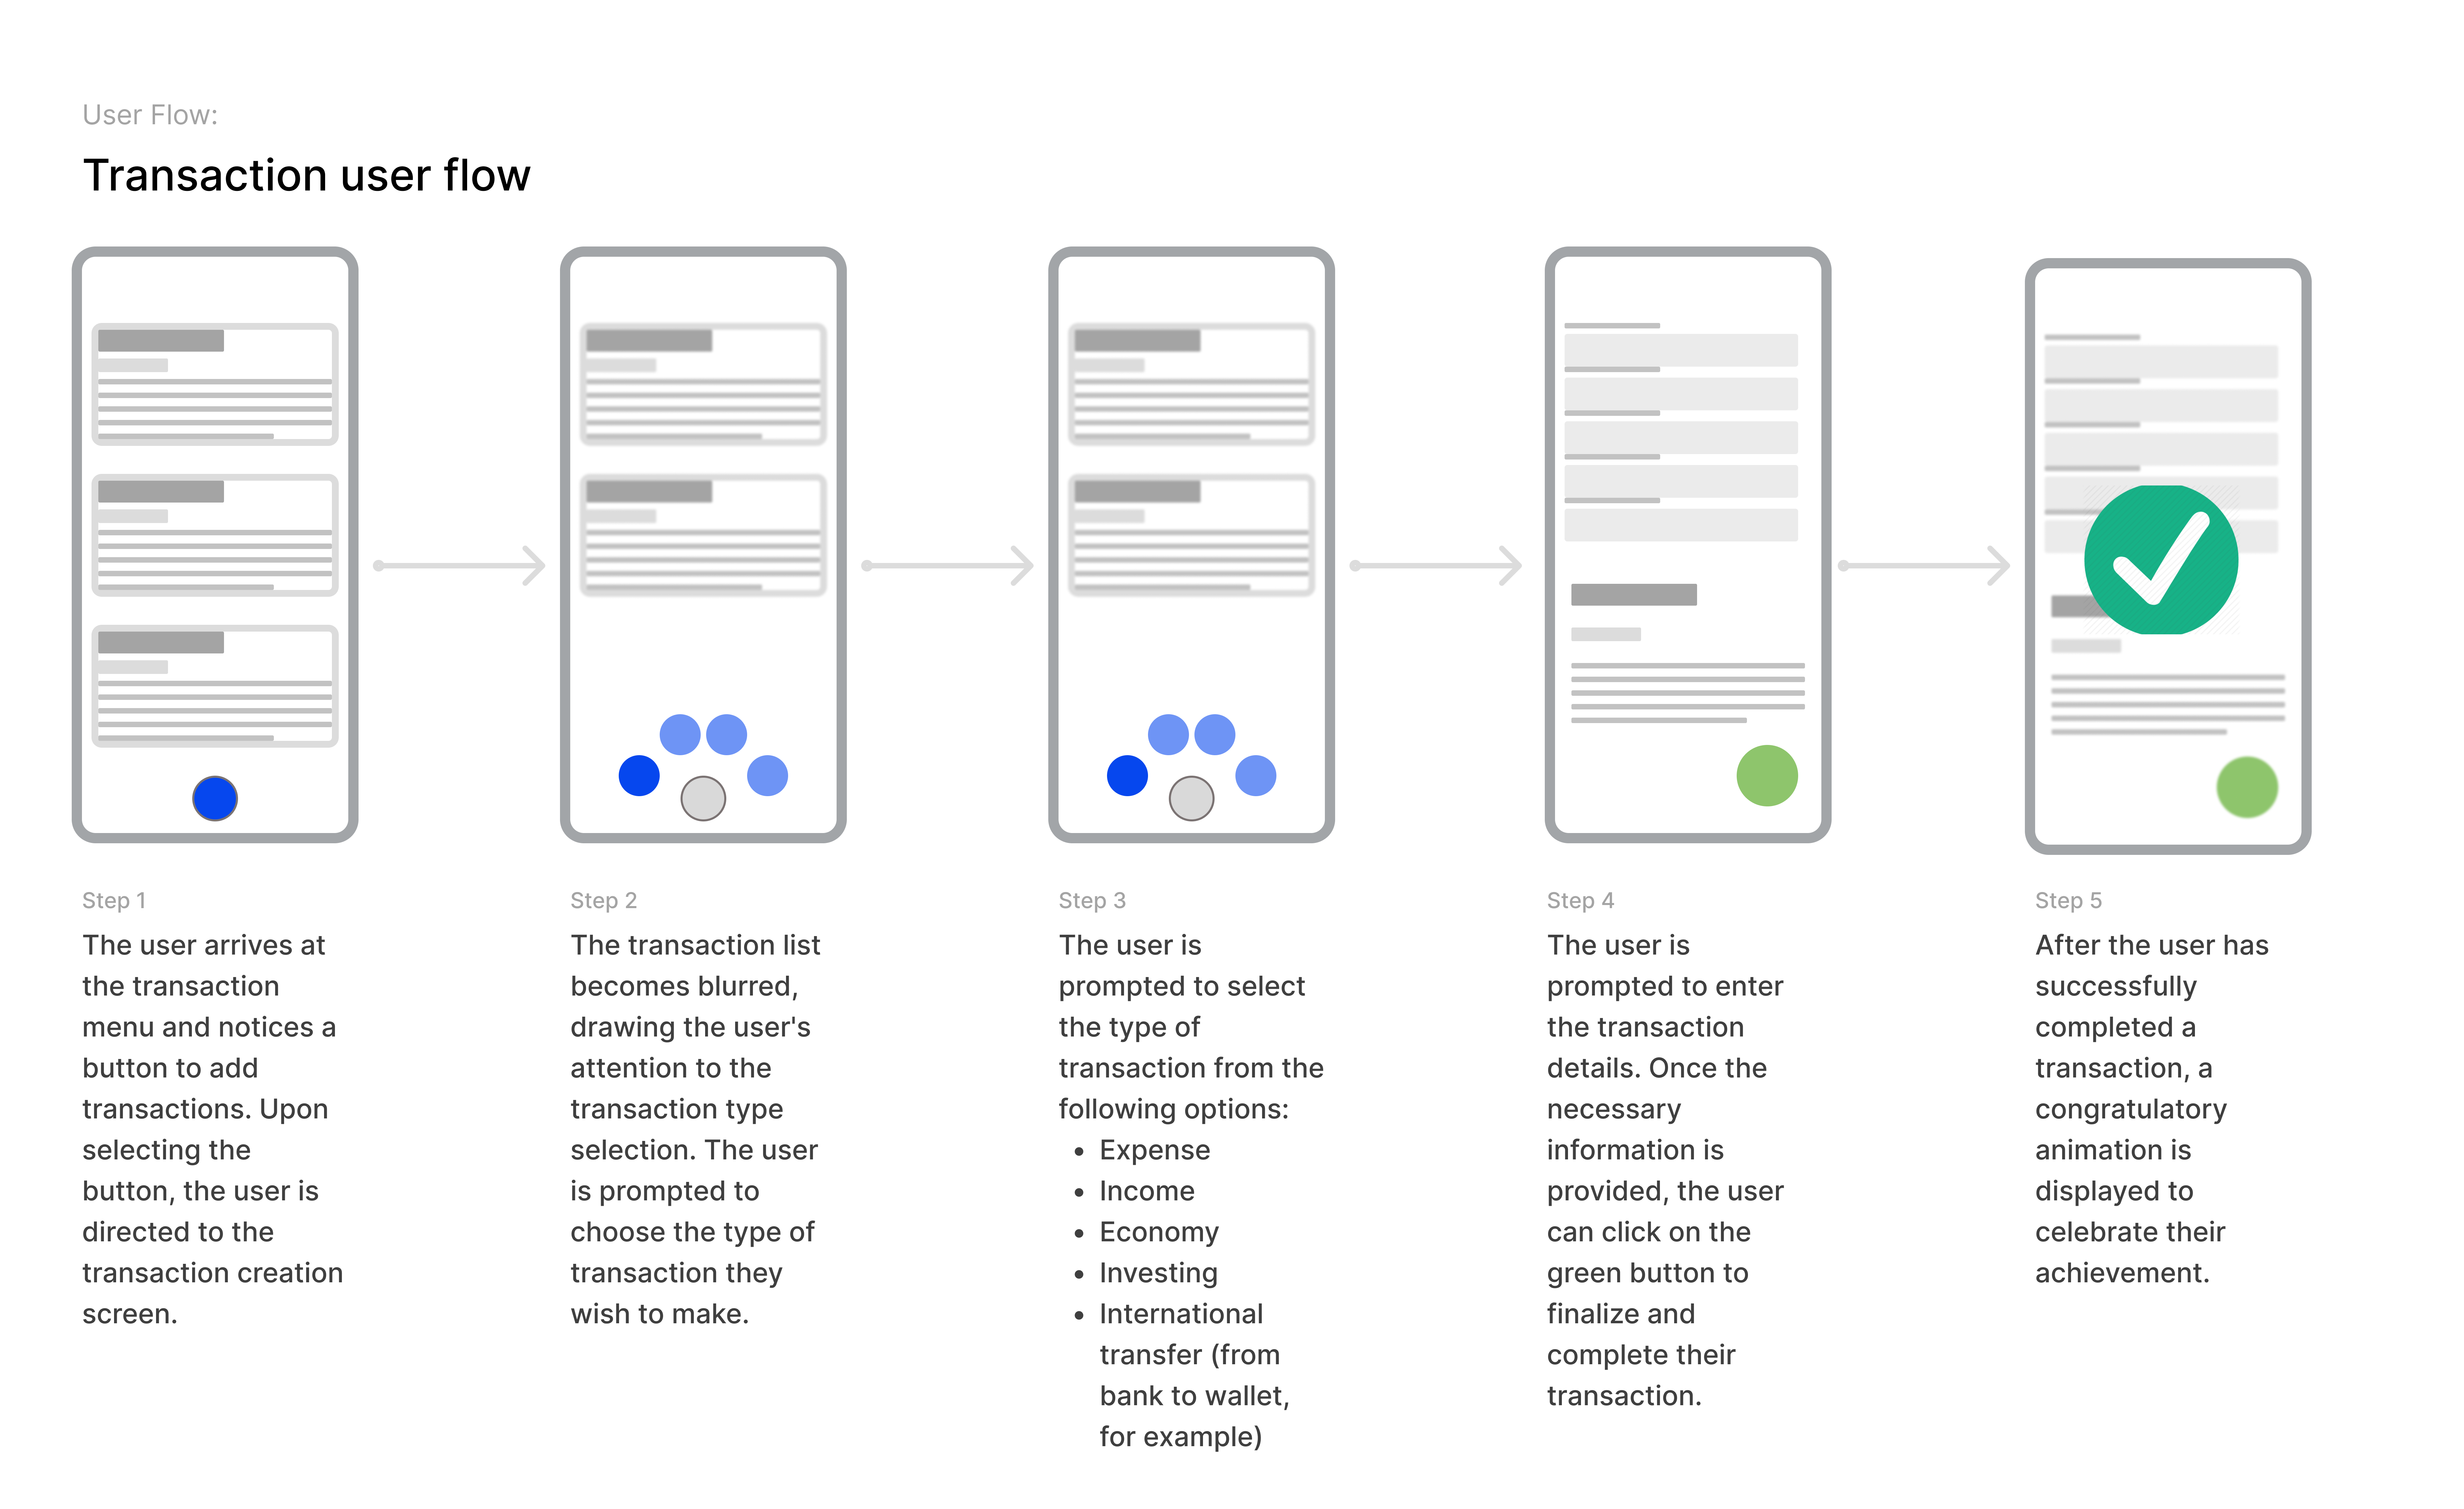
\includegraphics[width=\textwidth]{Graphics/UserFlows/TransactionUserFlow.png}
  \caption{User Flow for a Transaction}
  \label{fig:transaction_flow}
\end{figure}

Figure~\ref{fig:transaction_flow} illustrates the user flow for a transaction in a visual format. Users follow these steps to complete a transaction and ensure accurate record-keeping of their financial activities.

The transaction process is designed to be intuitive and user-friendly, allowing users to quickly and efficiently record their expenses and income within the app.

\newpage
\section{Application Screens}
\begin{itemize}
\item Login Screen: Users can access the app by entering their login credentials on this screen (Figure \ref{fig:login}).
\item Login Error - Password Missing: This screen indicates an error during the login process due to a missing password (Figure \ref{fig:login-error}).
\end{itemize}

\begin{figure}[htbp]
    \centering
    \begin{minipage}[t]{0.35\textwidth}
        \centering
        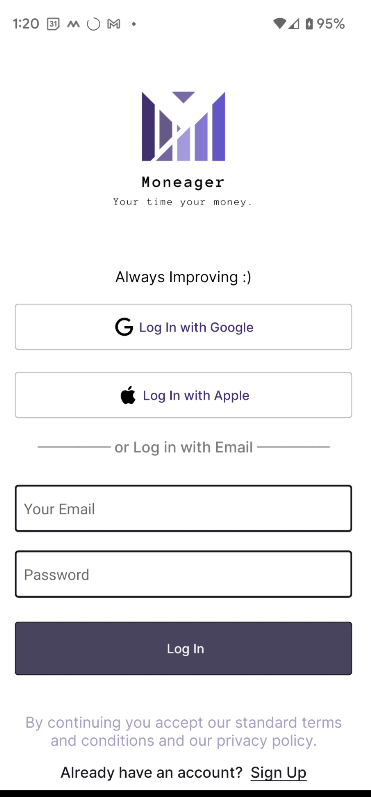
\includegraphics[width=\textwidth]{Screen Shots/Moneager/ScreenShotLogin.png}
        \caption{Login Screen}
        \label{fig:login}
    \end{minipage}
    \hfill
    \begin{minipage}[t]{0.35\textwidth}
        \centering
        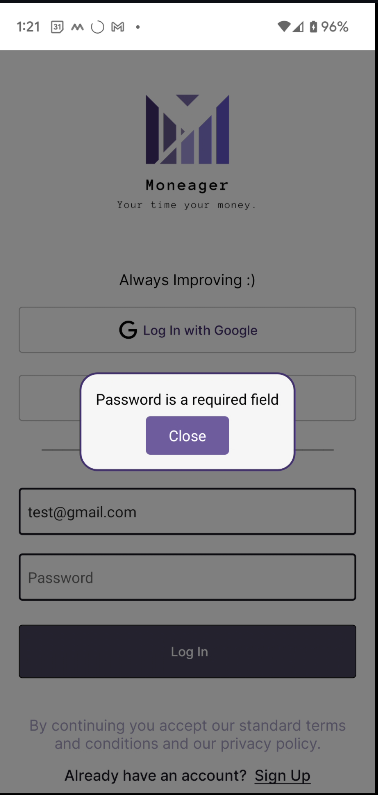
\includegraphics[width=\textwidth]{Screen Shots/Moneager/ScreenShotLoginErrorPasswordMissing.png}
        \caption{Login Error - Password Missing}
        \label{fig:login-error}
    \end{minipage}
\end{figure}

\begin{itemize}
\item Register Screen: This screen presents a user registration form where new users can provide their information to create an account (Figure \ref{fig:register}).
\item User Registration Error: This screen alerts users about an error that occurred during the registration process due to invalid user registration data (Figure \ref{fig:registration-error}).
\end{itemize}

\begin{figure}[htbp]
    \centering
    \begin{minipage}[t]{0.35\textwidth}
        \centering
        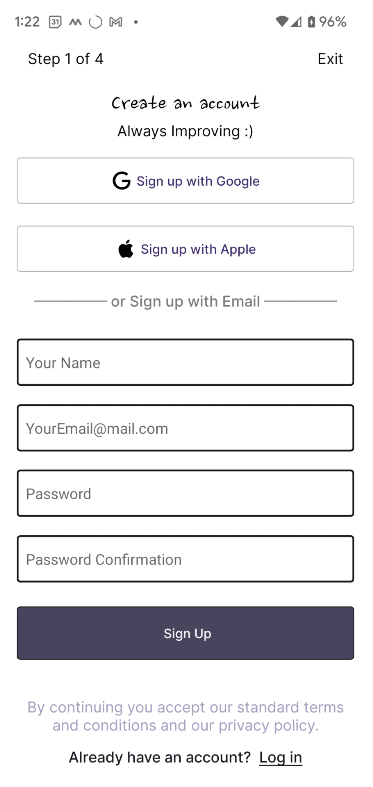
\includegraphics[width=\textwidth]{Screen Shots/Moneager/RegisterScreen.png}
        \caption{Register Screen}
        \label{fig:register}
    \end{minipage}
    \hfill
    \begin{minipage}[t]{0.35\textwidth}
        \centering
        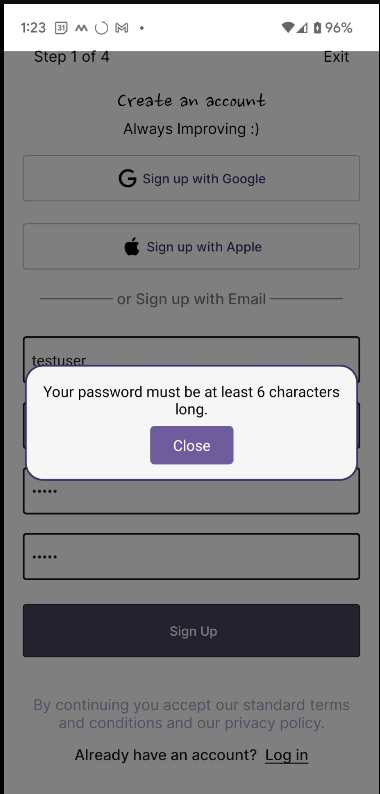
\includegraphics[width=\textwidth]{Screen Shots/Moneager/ScreenShotRegisterUserError.png}
        \caption{User Registration Error}
        \label{fig:registration-error}
    \end{minipage}
\end{figure}

\newpage
\subsection{Transaction Screens}

\begin{itemize}
\item Transaction History Screen: This screen provides a comprehensive list of the user's past transactions (Figure \ref{fig:transaction-history}).
\item Transaction Creator Screen: This screen enables users to create new transactions (Figure \ref{fig:transaction-creator}).
\item Invalid Transaction Example: This screen displays an error message when the user attempts to enter an invalid transaction (Figure \ref{fig:invalid-transaction}).
\end{itemize}

\begin{figure}[htbp]
    \centering
    \begin{minipage}[t]{0.2\textwidth}
        \centering
        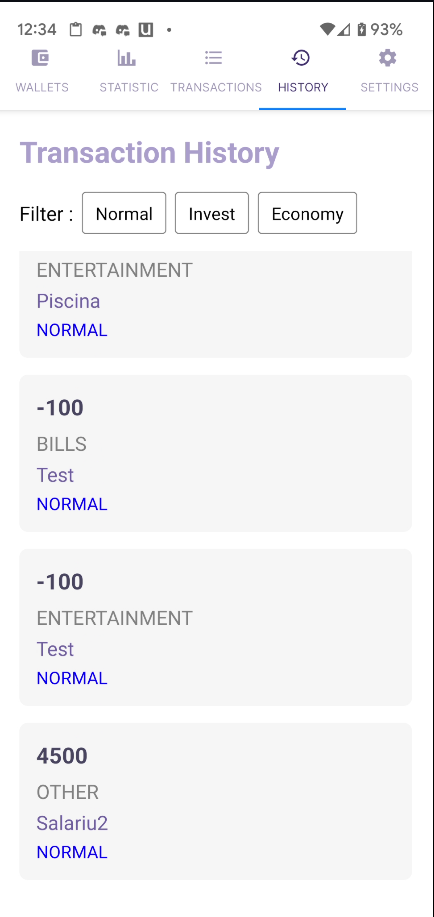
\includegraphics[width=\textwidth]{Screen Shots/Moneager/TranasactionHistoryScreen.png}
        \caption{Transaction History Screen}
        \label{fig:transaction-history}
    \end{minipage}
    \hfill
    \begin{minipage}[t]{0.2\textwidth}
        \centering
        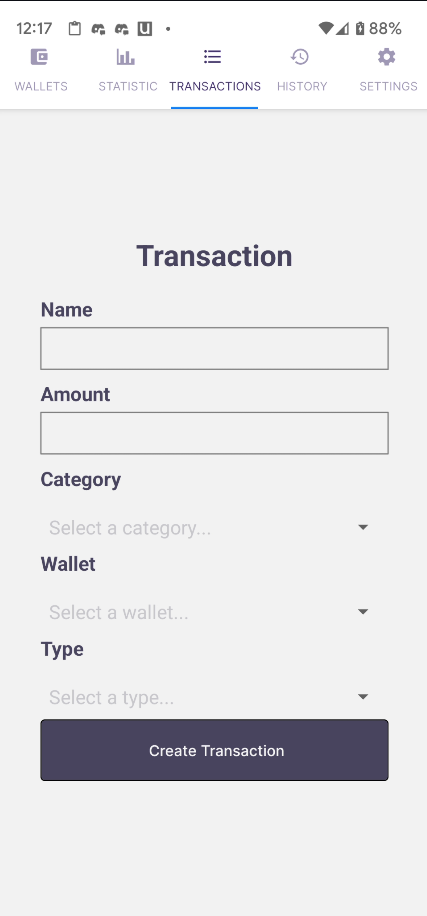
\includegraphics[width=\textwidth]{Screen Shots/Moneager/TransanctionCreatorScreen.png}
        \caption{Transaction Creator Screen}
        \label{fig:transaction-creator}
    \end{minipage}
    \hfill
    \begin{minipage}[t]{0.2\textwidth}
        \centering
        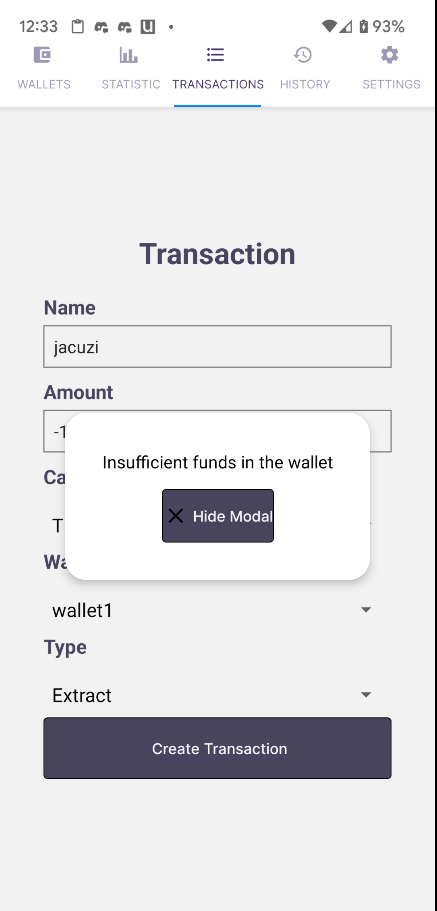
\includegraphics[width=\textwidth]{Screen Shots/Moneager/Inavlid Transaction Example.png}
        \caption{Invalid Transaction Example}
        \label{fig:invalid-transaction}
    \end{minipage}
\end{figure}


\subsection{Additional Screens}

\begin{itemize}
\item Transaction Screen Screen: This screen serves as the app's transaction creator screen (Figure \ref{fig:main-menu}).
\item Settings Screen: This screen allows the user to modify the settings of the application (Figure \ref{fig:settings}).
\item Statistics Screen: Users can see a statistical overview of their financial activities on this screen (Figure \ref{fig:statistics}).
\item Wallet Balance Screen: This screen displays the current balance of the user's wallet (Figure \ref{fig:wallet-balance}).
\end{itemize}

\begin{figure}[htbp]
    \centering
    \begin{minipage}[t]{0.2\textwidth}
        \centering
        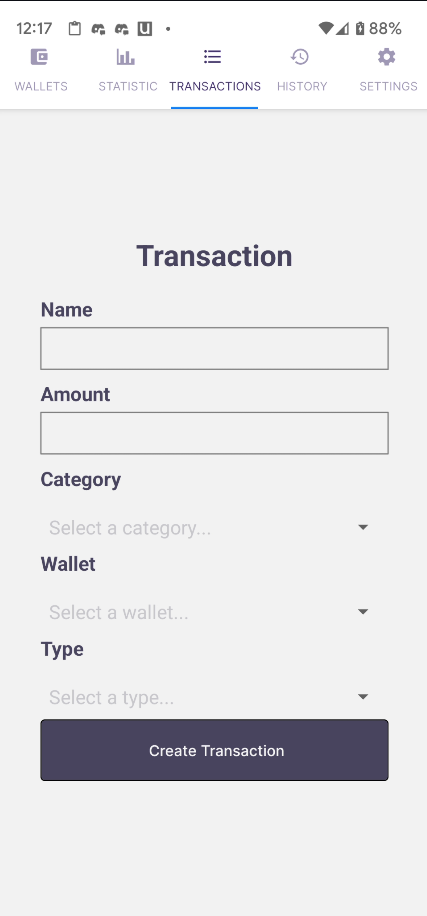
\includegraphics[width=\textwidth]{Screen Shots/Moneager/TransanctionCreatorScreen.png}
        \caption{Transaction Screen}
        \label{fig:main-menu}
    \end{minipage}
    \hfill
    \begin{minipage}[t]{0.2\textwidth}
        \centering
        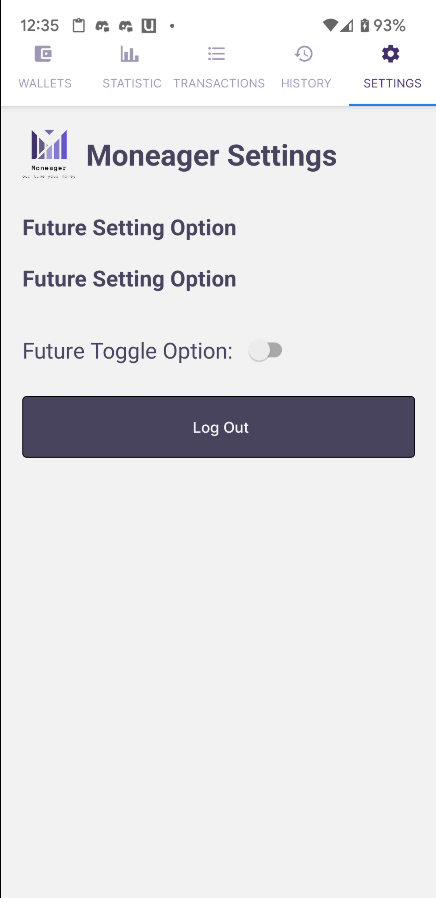
\includegraphics[width=\textwidth]{Screen Shots/Moneager/SettingsScreen.png}
        \caption{Settings Screen}
        \label{fig:settings}
    \end{minipage}
    \hfill
    \begin{minipage}[t]{0.2\textwidth}
        \centering
        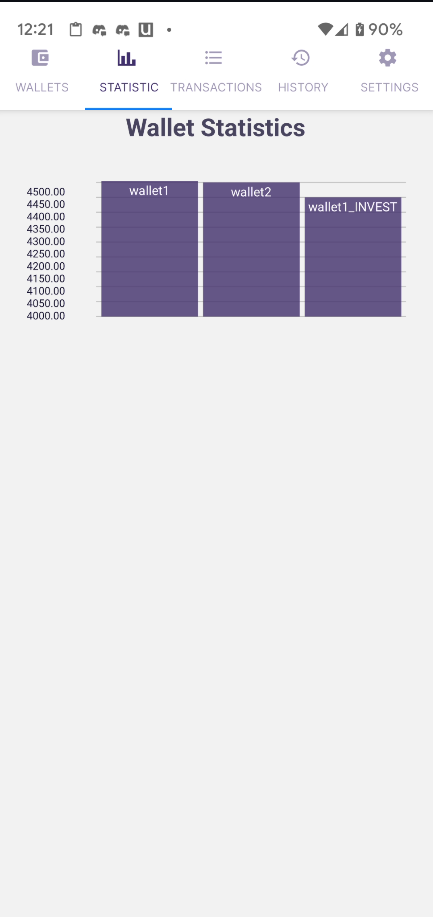
\includegraphics[width=\textwidth]{Screen Shots/Moneager/StatisticsScreen.png}
        \caption{Statistics Screen}
        \label{fig:statistics}
    \end{minipage}
    \hfill
    \begin{minipage}[t]{0.2\textwidth}
        \centering
        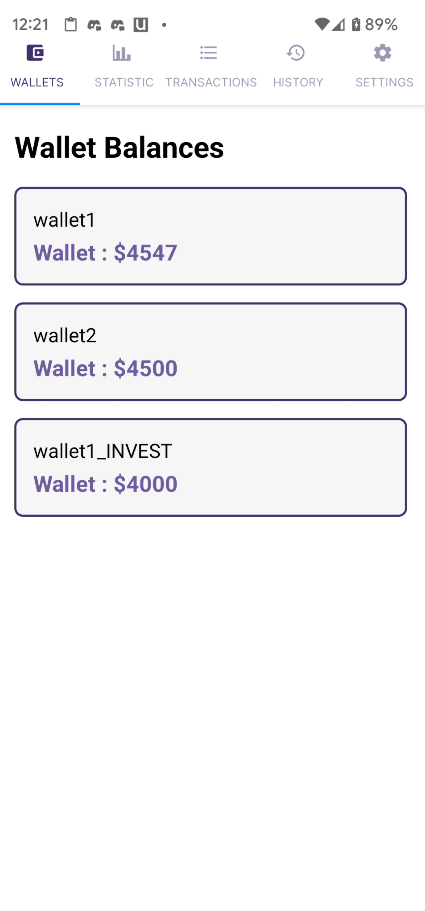
\includegraphics[width=\textwidth]{Screen Shots/Moneager/WalletBalanceScreen.png}
        \caption{Wallet Balance Screen}
        \label{fig:wallet-balance}
    \end{minipage}
\end{figure}


% \section{Onboarding Screens}

% \begin{itemize}
% \item Onboarding Screen 1: This screen welcomes new users to the Money Manager app and provides a brief introduction to its features (Figure \ref{fig:onb1}).
% \item Onboarding Screen 2: This screen highlights key features and benefits of the app, encouraging users to explore further (Figure \ref{fig:onb2}).
% \item Onboarding Screen 3: Users are prompted to select their preferences and customize the app according to their needs (Figure \ref{fig:onb3}).
% \item Onboarding Screen 4: This screen allows users to create a new account by providing their registration details (Figure \ref{fig:onb4}).
% \item Onboarding Screen 5: Users receive a completion message, indicating the successful completion of the onboarding process (Figure \ref{fig:onb5}).
% \end{itemize}

% \begin{figure}[htbp]
%     \centering
%     \begin{minipage}[t]{0.2\textwidth}
%         \centering
%         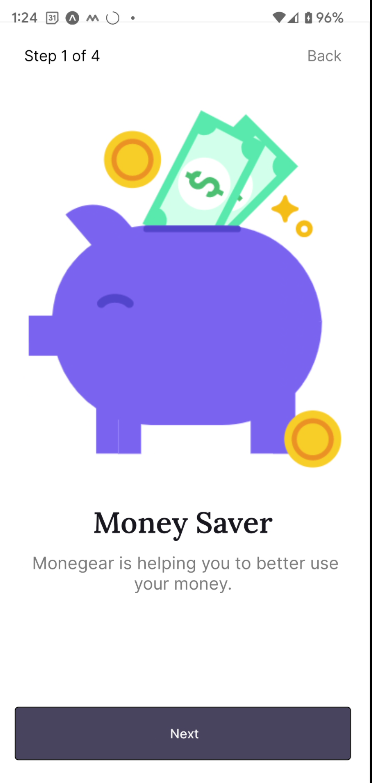
\includegraphics[width=\textwidth]{Screen Shots/Moneager/Onb1.png}
%         \caption{Onboarding Screen 1}
%         \label{fig:onb1}
%     \end{minipage}
%     \hfill
%     \begin{minipage}[t]{0.2\textwidth}
%         \centering
%         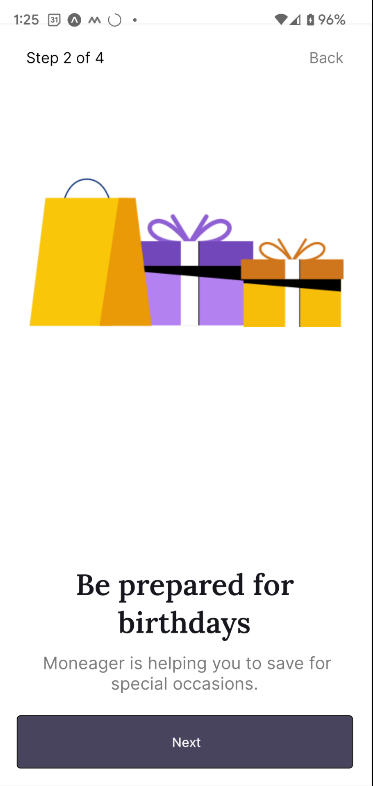
\includegraphics[width=\textwidth]{Screen Shots/Moneager/Onb2.png}
%         \caption{Onboarding Screen 2}
%         \label{fig:onb2}
%     \end{minipage}
%     \begin{minipage}[t]{0.2\textwidth}
%         \centering
%         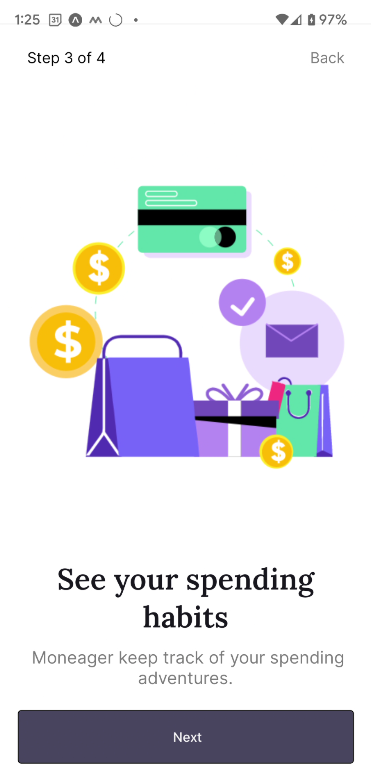
\includegraphics[width=\textwidth]{Screen Shots/Moneager/Onb3.png}
%         \caption{Onboarding Screen 3}
%         \label{fig:onb3}
%     \end{minipage}
%     \hfill
%     \begin{minipage}[t]{0.2\textwidth}
%         \centering
%         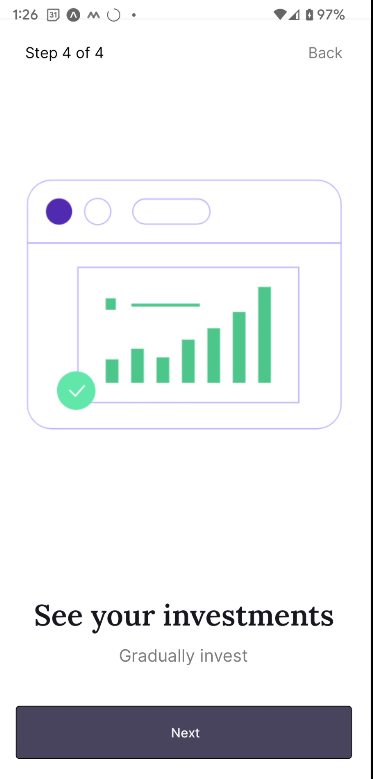
\includegraphics[width=\textwidth]{Screen Shots/Moneager/Onb4.png}
%         \caption{Onboarding Screen 4}
%         \label{fig:onb4}
%     \end{minipage}
%     \begin{minipage}[t]{0.2\textwidth}
%         \centering
%         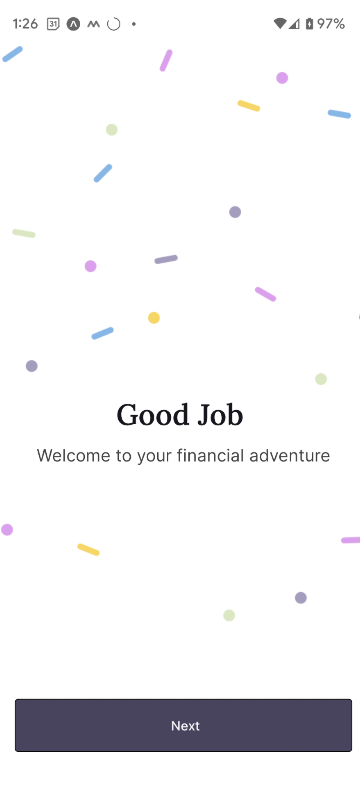
\includegraphics[width=\textwidth]{Screen Shots/Moneager/Onb5.png}
%         \caption{Onboarding Screen 5}
%         \label{fig:onb5}
%     \end{minipage}
% \end{figure}



% In this section, we will provide descriptions of the screen displays captured from the Money Manager application. These screen displays showcase various user interfaces and functionalities of the app. Each image represents a specific screen within the application, and we will provide a brief description of the purpose and features of each screen.

% \textbf{Onboarding Screens}:
% \begin{itemize}
% \item \textbf{Onboarding Screen 1} (Figure \ref{fig:onb1}): This screen welcomes new users to the Money Manager app and provides a brief introduction to its features.
% \item \textbf{Onboarding Screen 2} (Figure \ref{fig:onb2}): This screen highlights key features and benefits of the app, encouraging users to explore further.
% \item \textbf{Onboarding Screen 3} (Figure \ref{fig:onb3}): Users are prompted to select their preferences and customize the app according to their needs.
% \item \textbf{Onboarding Screen 4} (Figure \ref{fig:onb4}): This screen allows users to create a new account by providing their registration details.
% \item \textbf{Onboarding Screen 5} (Figure \ref{fig:onb5}): Users receive a completion message, indicating the successful completion of the onboarding process.
% \item \textbf{Register Screen} (Figure \ref{fig:register}): This screen presents a user registration form where new users can provide their information to create an account.
% \end{itemize}

% \textbf{Other Screens}:
% \begin{itemize}
% \item \textbf{Login Error - Password Missing} (Figure \ref{fig:login-error}): This screen indicates an error during the login process due to a missing password.
% \item \textbf{Login Screen} (Figure \ref{fig:login}): Users can access the app by entering their login credentials on this screen.
% \item \textbf{Main Menu Screen} (Figure \ref{fig:main-menu}): This screen serves as the app's main menu, providing navigation options and an overview of its features.
% \item \textbf{User Registration Error} (Figure \ref{fig:registration-error}): This screen alerts users about an error that occurred during the registration process due to invalid user registration data.
% \item \textbf{Invalid Transaction Example} (Figure \ref{fig:invalid-transaction}): This screen displays an error message when the user attempts to enter an invalid transaction.
% \item \textbf{Settings Screen} (Figure \ref{fig:settings}): This screen allows the user to modify the settings of the application.
% \item \textbf{Statistics Screen} (Figure \ref{fig:statistics}): Users can see a statistical overview of their financial activities on this screen.
% \item \textbf{Transaction History Screen} (Figure \ref{fig:transaction-history}): This screen provides a comprehensive list of the user's past transactions.
% \item \textbf{Transaction Creator Screen} (Figure \ref{fig:transaction-creator}): This screen enables users to create new transactions.
% \item \textbf{Wallet Balance Screen} (Figure \ref{fig:wallet-balance}): This screen displays the current balance of the user's wallet.
% \end{itemize}

% \begin{figure}[htbp]
%     \centering

%     \begin{minipage}[t]{0.4\textwidth}
%         \centering
%         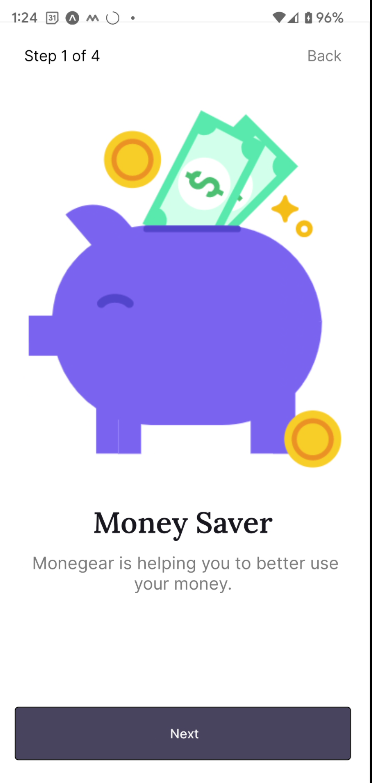
\includegraphics[width=\textwidth]{Screen Shots/Moneager/Onb1.png}
%         \caption{Onboarding Screen 1}
%         \label{fig:onb1}
%     \end{minipage}
%     \hfill
%     \begin{minipage}[t]{0.4\textwidth}
%         \centering
%         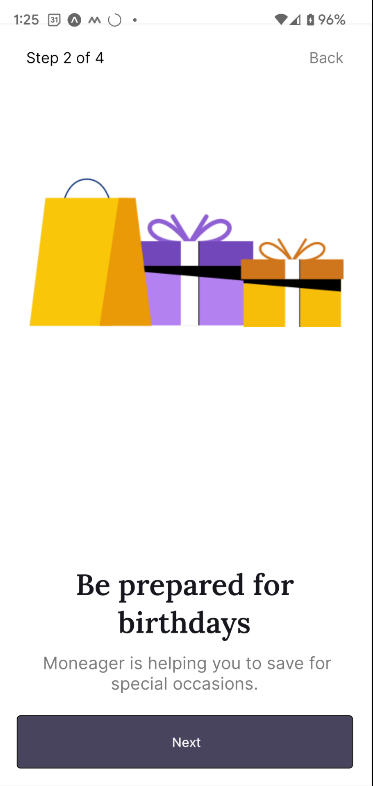
\includegraphics[width=\textwidth]{Screen Shots/Moneager/Onb2.png}
%         \caption{Onboarding Screen 2}
%         \label{fig:onb2}
%     \end{minipage}
% \end{figure}

% \begin{figure}[htbp]
%     \centering

%     \begin{minipage}[t]{0.4\textwidth}
%         \centering
%         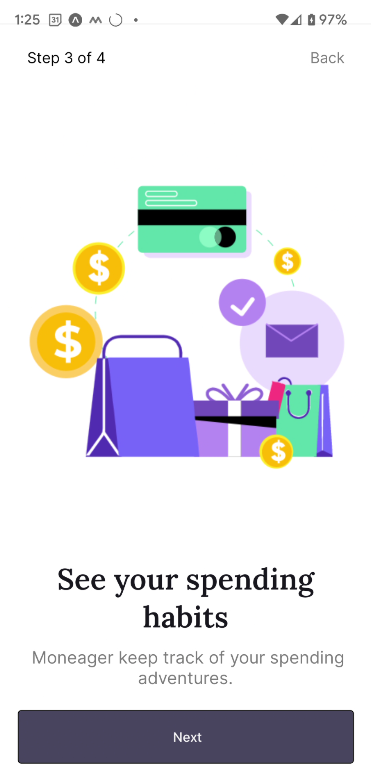
\includegraphics[width=\textwidth]{Screen Shots/Moneager/Onb3.png}
%         \caption{Onboarding Screen 3}
%         \label{fig:onb3}
%     \end{minipage}
%     \hfill
%     \begin{minipage}[t]{0.4\textwidth}
%         \centering
%         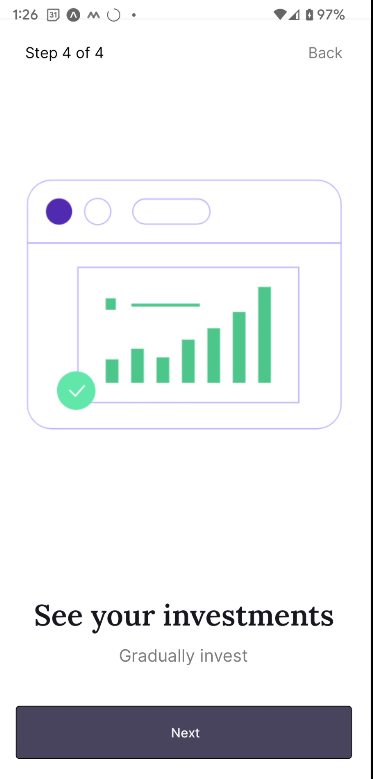
\includegraphics[width=\textwidth]{Screen Shots/Moneager/Onb4.png}
%         \caption{Onboarding Screen 4}
%         \label{fig:onb4}
%     \end{minipage}
% \end{figure}

% \begin{figure}[htbp]
%     \centering

%     \begin{minipage}[t]{0.4\textwidth}
%         \centering
%         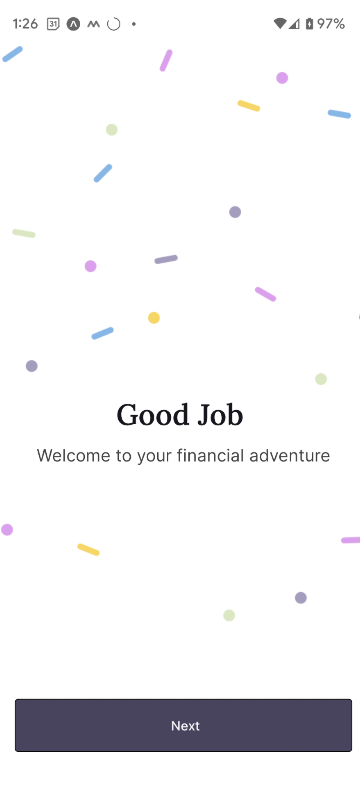
\includegraphics[width=\textwidth]{Screen Shots/Moneager/Onb5.png}
%         \caption{Onboarding Screen 5}
%         \label{fig:onb5}
%     \end{minipage}
%     \hfill
%     \begin{minipage}[t]{0.4\textwidth}
%         \centering
%         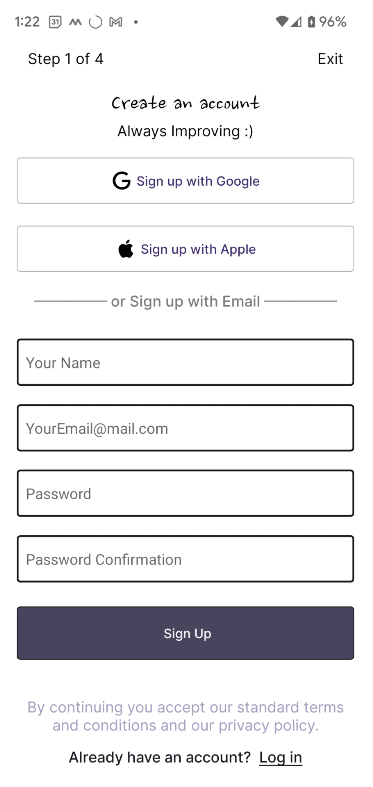
\includegraphics[width=\textwidth]{Screen Shots/Moneager/RegisterScreen.png}
%         \caption{Register Screen}
%         \label{fig:register}
%     \end{minipage}
% \end{figure}

% \begin{figure}[htbp]
%     \centering

%     \begin{minipage}[t]{0.4\textwidth}
%         \centering
%         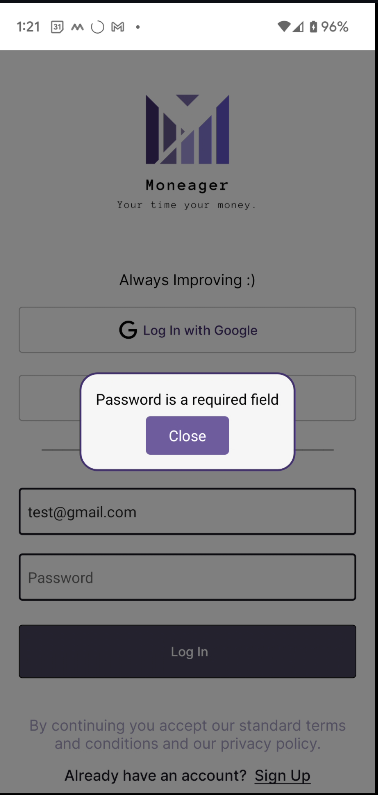
\includegraphics[width=\textwidth]{Screen Shots/Moneager/ScreenShotLoginErrorPasswordMissing.png}
%         \caption{Login Error - Password Missing}
%         \label{fig:login-error}
%     \end{minipage}
%     \hfill
%     \begin{minipage}[t]{0.4\textwidth}
%         \centering
%         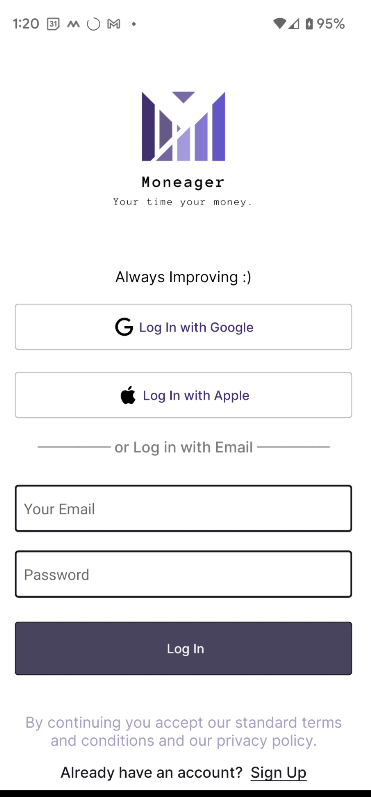
\includegraphics[width=\textwidth]{Screen Shots/Moneager/ScreenShotLogin.png}
%         \caption{Login Screen}
%         \label{fig:login}
%     \end{minipage}
% \end{figure}

% \begin{figure}[htbp]
%     \centering

%     \begin{minipage}[t]{0.4\textwidth}
%         \centering
%         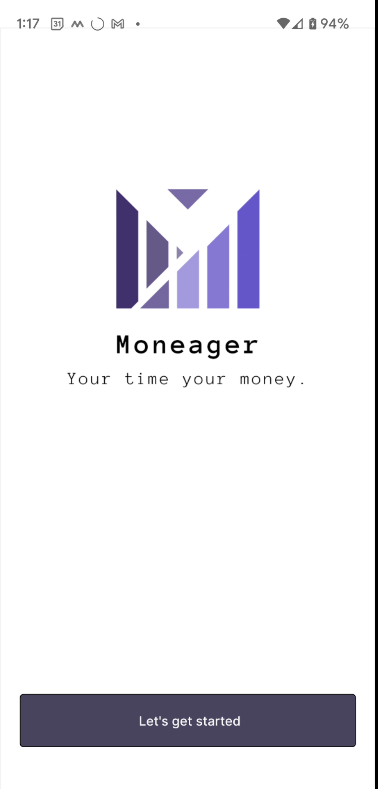
\includegraphics[width=\textwidth]{Screen Shots/Moneager/ScreenShotMainMenu.png}
%         \caption{Main Menu Screen}
%         \label{fig:main-menu}
%     \end{minipage}
%     \hfill
%     \begin{minipage}[t]{0.4\textwidth}
%         \centering
%         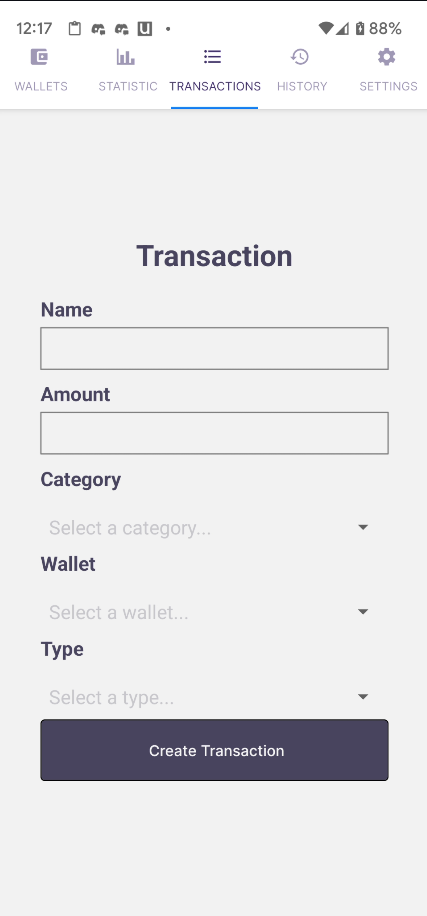
\includegraphics[width=\textwidth]{Screen Shots/Moneager/TransanctionCreatorScreen.png}
%         \caption{Transaction Creator Screen}
%         \label{fig:transaction-creator}
%     \end{minipage}
% \end{figure}

% \begin{figure}[htbp]
%     \centering

%     \begin{minipage}[t]{0.4\textwidth}
%         \centering
%         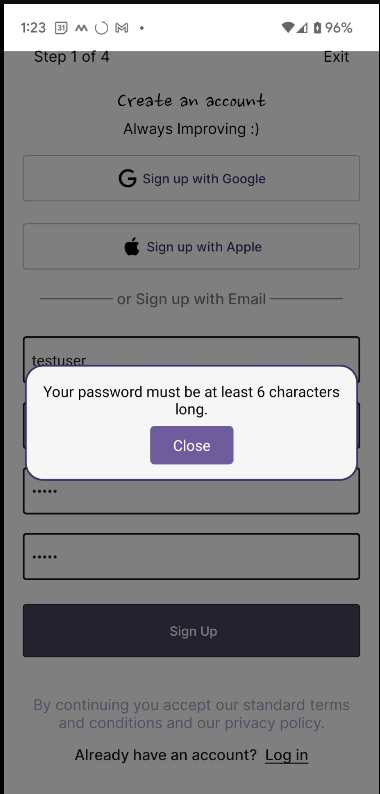
\includegraphics[width=\textwidth]{Screen Shots/Moneager/ScreenShotRegisterUserError.png}
%         \caption{User Registration Error}
%         \label{fig:registration-error}
%     \end{minipage}
%     \hfill
%     \begin{minipage}[t]{0.4\textwidth}
%         \centering
%         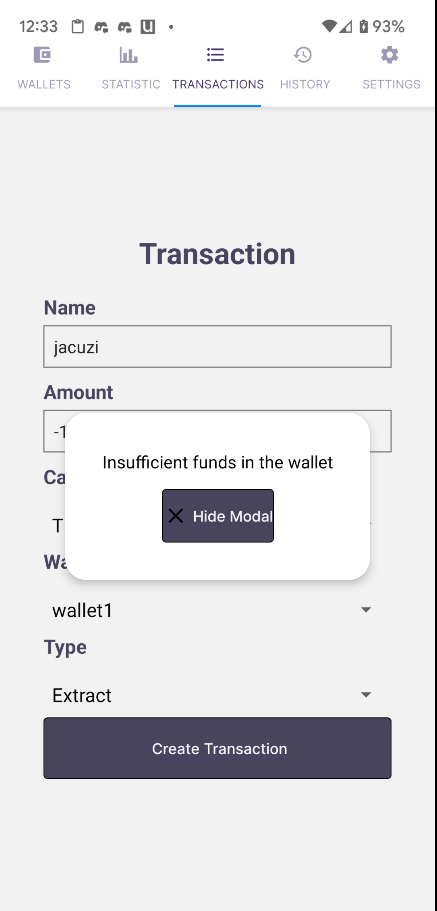
\includegraphics[width=\textwidth]{Screen Shots/Moneager/Inavlid Transaction Example.png}
%         \caption{Invalid Transaction Example}
%         \label{fig:invalid-transaction}
%     \end{minipage}
% \end{figure}

% \begin{figure}[htbp]
%     \centering

%     \begin{minipage}[t]{0.4\textwidth}
%         \centering
%         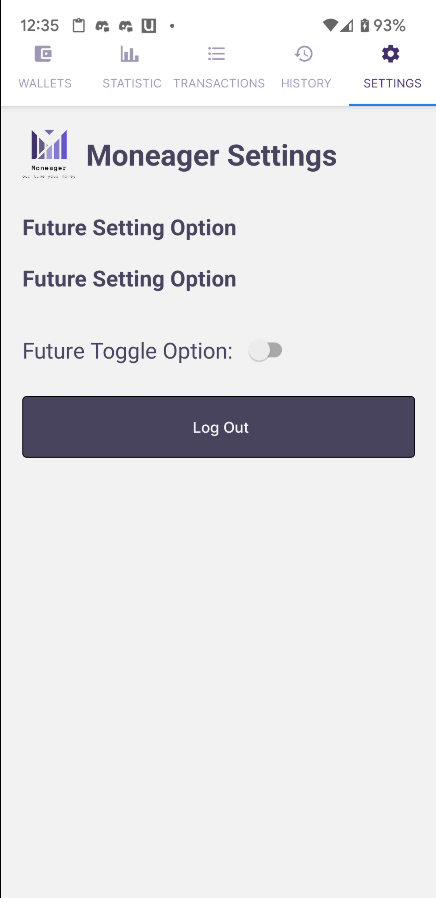
\includegraphics[width=\textwidth]{Screen Shots/Moneager/SettingsScreen.png}
%         \caption{Settings Screen}
%         \label{fig:settings}
%     \end{minipage}
%     \hfill
%     \begin{minipage}[t]{0.4\textwidth}
%         \centering
%         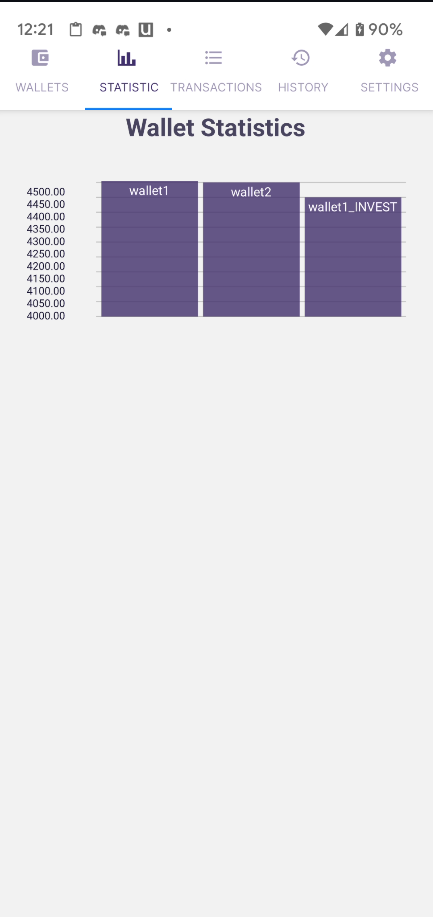
\includegraphics[width=\textwidth]{Screen Shots/Moneager/StatisticsScreen.png}
%         \caption{Statistics Screen}
%         \label{fig:statistics}
%     \end{minipage}
% \end{figure}

% \begin{figure}[htbp]
%     \centering
%     \begin{minipage}[t]{0.4\textwidth}
%         \centering
%         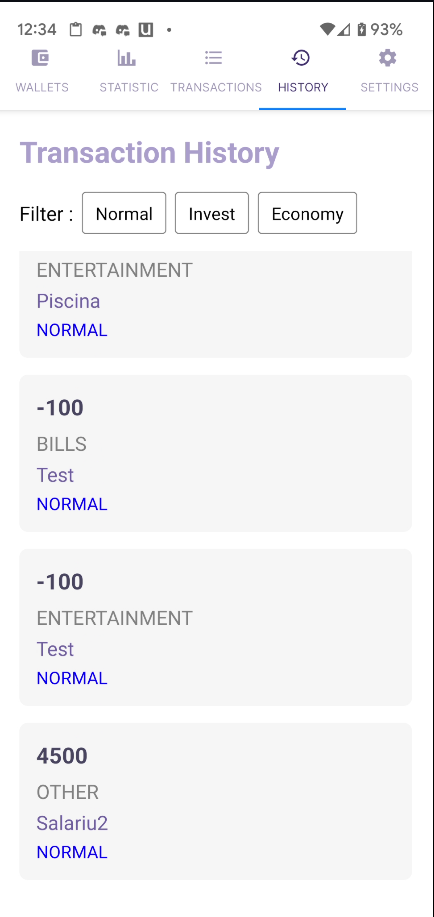
\includegraphics[width=\textwidth]{Screen Shots/Moneager/TranasactionHistoryScreen.png}
%         \caption{Transaction History Screen}
%         \label{fig:transaction-history}
%     \end{minipage}
%     \hfill
%     \begin{minipage}[t]{0.4\textwidth}
%         \centering
%         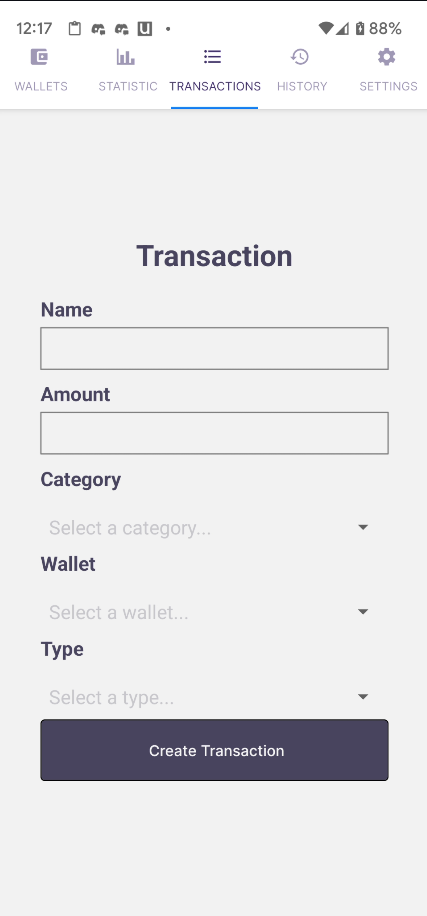
\includegraphics[width=\textwidth]{Screen Shots/Moneager/TransanctionCreatorScreen.png}
%         \caption{Transaction Creator Screen}
%         \label{fig:transaction-creator}
%     \end{minipage}
% \end{figure}

% \begin{figure}[htbp]
%     \centering
%     \begin{minipage}[t]{0.4\textwidth}
%         \centering
%         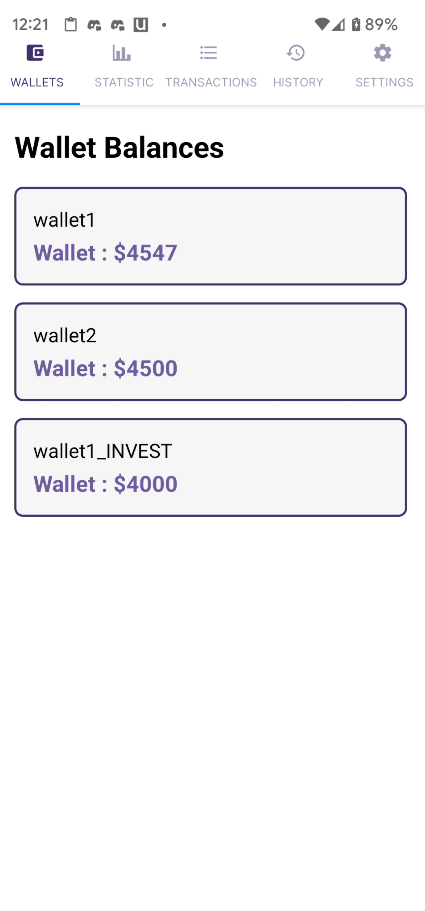
\includegraphics[width=\textwidth]{Screen Shots/Moneager/WalletBalanceScreen.png}
%         \caption{Wallet Balance Screen}
%         \label{fig:wallet-balance}
%     \end{minipage}
% \end{figure}



% \newpage

\section{Project Structure}

The provided directory structure represents the organization of files and folders in the front-end development of the application. It encompasses essential aspects such as assets, components, constants, navigation, and services. This structured approach facilitates modularity, code re-usability, and maintainability, enabling developers to effectively manage resources and functionalities throughout the development process.

It is important to note that only a subset of files and folders are shown in the provided structure for the sake of feasibility. The actual structure may include additional files and folders depending on the specific requirements of the project. The shown files provide an overview of the key elements present in the front-end development, while other supporting files and folders are assumed to be present to ensure the smooth functioning of the application.


\begin{itemize}
  \item \texttt{assets}: The \texttt{assets} folder is used to store various asset files such as images, icons, and splash screens.
    \begin{itemize}
      \item \texttt{images}: This subfolder within \texttt{assets} is specifically used to store different images used in the application.
    \end{itemize}
  \item \texttt{components}: The \texttt{components} folder contains different components used in the application.
    \begin{itemize}
      \item \texttt{screens}: This subfolder within \texttt{components} is dedicated to screen components.
      \item \texttt{shared}: This subfolder within \texttt{components} contains shared components.
      \item \texttt{ui}: This subfolder within \texttt{components} is specifically used for UI components.
    \end{itemize}
  \item \texttt{constants}: The \texttt{constants} folder is used to store files related to constants or configurations.
    \begin{itemize}
      \item \texttt{colors.tsx}: This file within the \texttt{constants} folder defines color constants used in the application.
      \item \texttt{fonts}: This subfolder within \texttt{constants} is dedicated to font-related files.
      \item \texttt{graphql}: This subfolder within \texttt{constants} is specifically used for GraphQL-related configurations.
    \end{itemize}
  \item \texttt{navigation}: The \texttt{navigation} folder contains files related to navigation within the application.
    \begin{itemize}
      \item \texttt{accountCreationStackNavigator.tsx}: This file defines the stack navigator specifically for the account creation process.
      \item \texttt{skect\_bottomTabNavigator.tsx}: This file defines the bottom tab navigator used for the application.
    \end{itemize}
  \item \texttt{services}: The \texttt{services} folder is used to store files related to various services or utilities.
    \begin{itemize}
      \item \texttt{AuthHandler.tsx}: This file within the \texttt{services} folder handles authentication-related functionality.
      \item \texttt{CustomResourceLoading.tsx}: This file within the \texttt{services} folder handles custom resource loading.
      \item \texttt{ErrorHandler}: This subfolder within \texttt{services} contains files related to error handling.
    \end{itemize}
\end{itemize}


\subsection{Applications core logic} 


The main UML diagram, as shown in Figure \ref{fig:transaction_flow}, provides an overview of the core logic and structure of the application. It represents the relationships and interactions between various components and modules, highlighting the flow of data and control within the system.

This comprehensive diagram serves as a visual representation of the application's architecture and helps developers and stakeholders gain a better understanding of how different components and modules interact with each other. It provides insights into the major functionalities, data flow, and dependencies within the system.

\begin{figure}[h!]
  \centering
  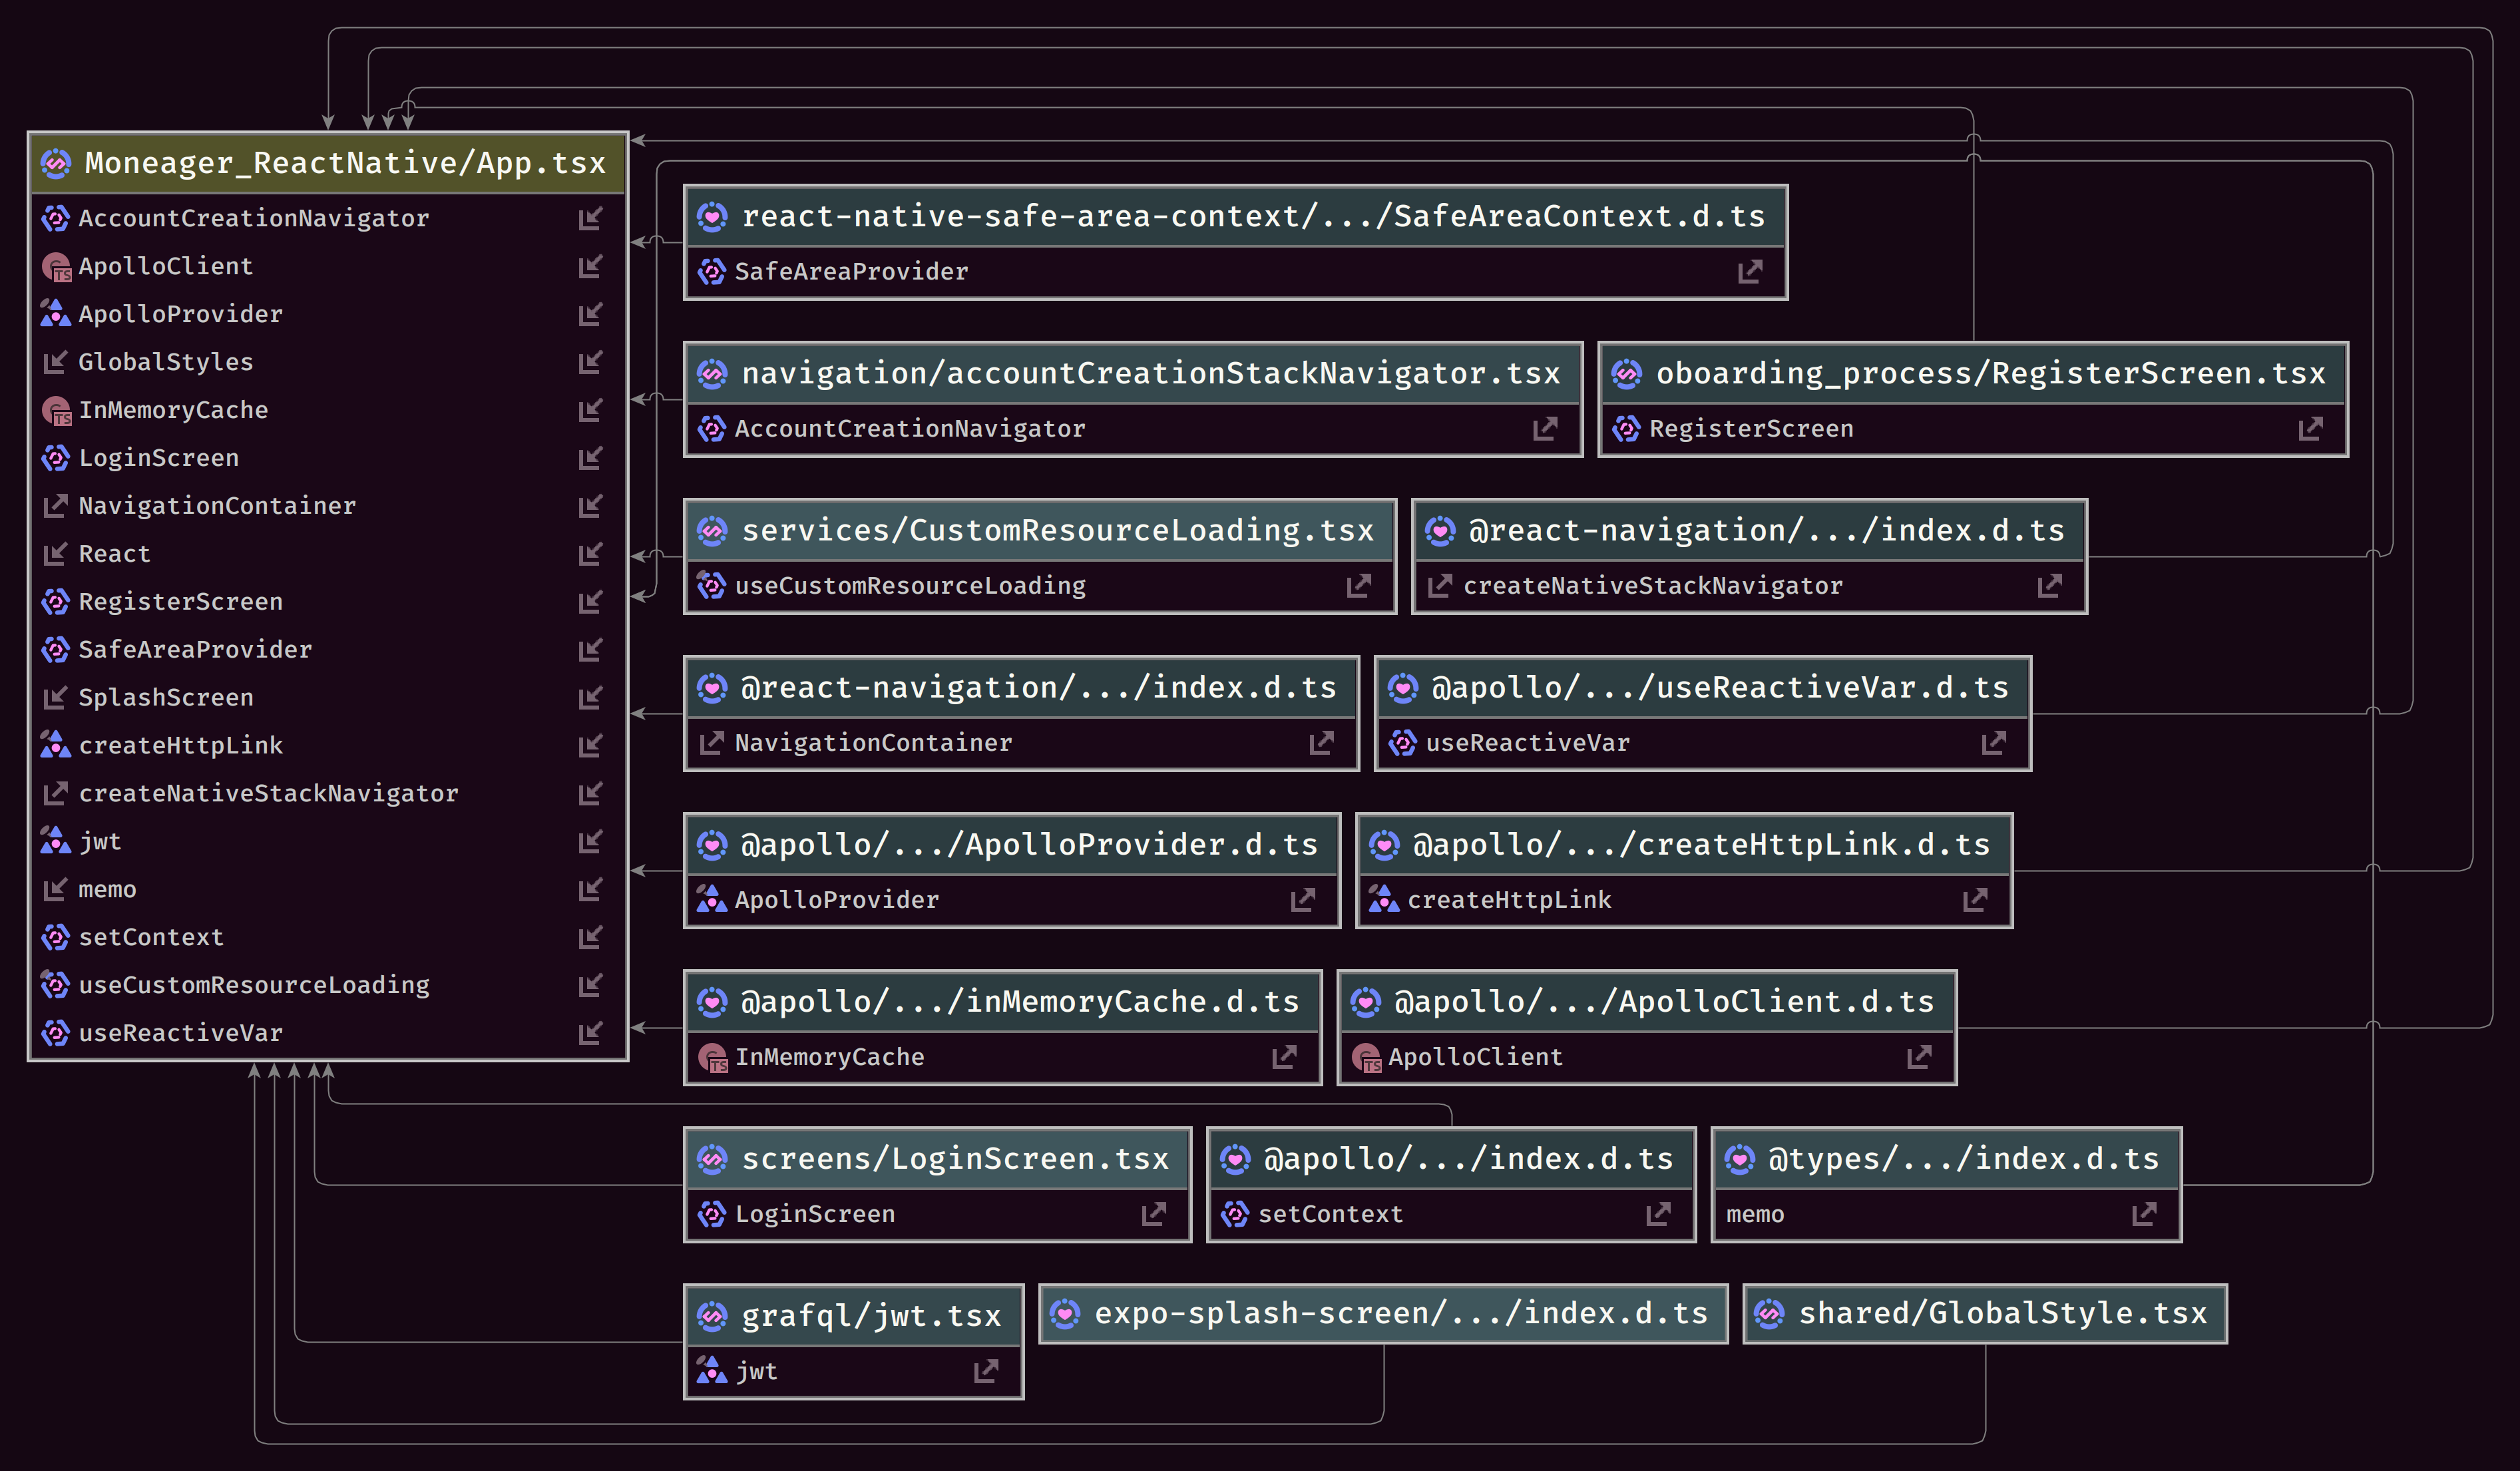
\includegraphics[width=\textwidth]{Diagram/MainDiagram.png}
  \caption{Main UML diagram}
  \label{fig:transaction_flow}
\end{figure}


The short outline diagram, shown in Figure \ref{fig:transaction_flow}, provides a condensed overview of the application's structure and major components. It offers a high-level representation of the key modules and their relationships, serving as a quick reference for understanding the overall architecture of the system.

\begin{figure}[h!]
  \centering
  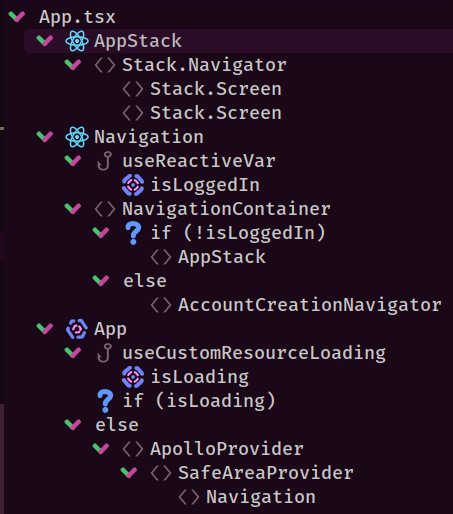
\includegraphics[width=0.4\textwidth]{Diagram/Outline/OutlineMain.png}
  \caption{Short Outline diagram}
  \label{fig:transaction_flow}
\end{figure}


In this subsection, the main file {App.tsx} is utilized and extended to create the core logic of the application. The {App.tsx} file serves as the entry point for the application and is responsible for initializing the required components and configuring the overall structure of the app. The code and its functionality can be described as follows:



\begin{lstlisting}[language=TypeScript]
// Backend Link
const authLink = setContext((_, { headers }) => {
    // Get the JWT token
    const token = jwt();
    return {
        headers: {
            ...headers,
            // Add the token to the Authorization header
            authorization: token ? `Bearer ${token}` : "",
        }
    }
});
\end{lstlisting}

The \textit{authLink} is a middleware function that adds the JWT token to the headers of outgoing requests. It uses the \textit{setContext} function from Apollo Link to modify the request headers and includes the token in the Authorization header.


\begin{lstlisting}[language=TypeScript]
// GraphQL Endpoint
const httpLink = createHttpLink({
    uri: 'http://your\_graphql\_server:1337/graphql',
});
\end{lstlisting}

The \textit{httpLink} defines the GraphQL endpoint URL where the client sends its requests. It uses the \textit{createHttpLink} function from Apollo Link to create a link that connects to the specified GraphQL server.


\begin{lstlisting}[language=TypeScript]
const Stack = createNativeStackNavigator();

// Remember the client Cache
const client = new ApolloClient({
    link: authLink.concat(httpLink),
    cache: new InMemoryCache()
});
\end{lstlisting}

The \textit{Stack} is a component from the React Navigation library that manages the navigation stack. The \textit{createNativeStackNavigator} function is used to create a stack navigator instance.

The \textit{client} is an instance of the \textit{ApolloClient} that provides the connection to the GraphQL server. It is configured with the \textit{authLink} and \textit{httpLink} to handle authentication and network requests. The cache is created using the \textit{InMemoryCache} class, which manages the client-side cache for storing query results.


\begin{lstlisting}[language=TypeScript]
// Prevent unnecessary redraws
export const AppStack = memo(() => {
    return (
        <Stack.Navigator>
            <Stack.Screen name="LoginScreen" component={LoginScreen} options={{ headerShown: false }}/>
            <Stack.Screen name="RegisterScreen" component={RegisterScreen} options={{ headerShown: false }}/>
        </Stack.Navigator>
    );
});
\end{lstlisting}

The \textit{AppStack} is a React component defined using the \textit{memo} function to optimize rendering performance by preventing unnecessary redraws. It represents the stack navigator for the app screens. It includes screen components for login and registration, where the \textit{headerShown} option is set to \textit{false} to hide the header.


\begin{lstlisting}[language=TypeScript]
// Navigation checker
export const Navigation = () => {
    const isLoggedIn = useReactiveVar(jwt);
    return (
        <NavigationContainer>
            {!isLoggedIn ? <AppStack/> : <AccountCreationNavigator/>}
        </NavigationContainer>
    );
}
\end{lstlisting}

The \textit{Navigation} component serves as the entry point for the app's navigation. It uses the \textit{NavigationContainer} component from React Navigation to wrap the app's navigation hierarchy. It conditionally renders the \textit{AppStack} component or the \textit{AccountCreationNavigator} component based on whether the user is logged in or not.

\begin{lstlisting}[language=TypeScript]
export default function App() {
    const isLoading = useCustomResourceLoading();

    return isLoading ? null : (
        <ApolloProvider client={client}>
            <SafeAreaProvider style={GlobalStyles.droidSafeArea}>
                <Navigation/>
            </SafeAreaProvider>
        </ApolloProvider>
    );
}
\end{lstlisting}

The \textit{App} component is the root component of the app. It wraps the app with the \textit{ApolloProvider} component from Apollo Client, providing the client instance as the GraphQL client for the app.

It also wraps the app with the \textit{SafeAreaProvider} component from \textit{react-native-safe-area-context} to handle safe area insets on different devices. The \textit{Navigation} component is rendered inside the \textit{SafeAreaProvider}.

The \textit{isLoading} variable is used to conditionally render \textit{null} during the initial loading of custom resources.

Overall, this code sets up the necessary components and configurations for Apollo Client, React Navigation, and the app's navigation structure. It handles authentication, network requests, and provides the necessary context for making GraphQL queries and mutations.

The \textit{useCustomResourceLoading} function is a custom React Hook that is designed to manage the loading of custom resources within a React application. This hook helps ensure that the necessary resources, such as fonts, are loaded before the application renders its content, providing a smoother user experience.

The code snippet demonstrates the implementation of the \textit{useCustomResourceLoading} function:

\begin{lstlisting}[language=TypeScript]
export const useCustomResourceLoading = () => {
    let [fontsLoaded] = useFonts({
        Inter_400Regular,
        Inter_500Medium,
        NanumBrushScript_400Regular,
        Lora_400Regular,
        Lora_600SemiBold,
    });
}
\end{lstlisting}

In this code block, the \textit{useFonts} hook is utilized from the \textit{expo-font} package. It is responsible for loading the specified custom fonts required by the application. The \textit{fontsLoaded} variable represents the loading state of the fonts.


\begin{lstlisting}[language=TypeScript]
const [appIsReady, setAppIsReady] = useState(false);

useEffect(() => {
    async function prepare() {
        try {
            await SplashScreen.preventAutoHideAsync();
        } catch (err) {
            console.warn(err);
        } finally {
            setAppIsReady(true);
        }
    }

    prepare();
}, []);
    return (!fontsLoaded || !appIsReady);
};
\end{lstlisting}


The \textit{appIsReady} state variable and its corresponding setter function, \textit{setAppIsReady}, are created using the \textit{useState} hook. Initially, the \textit{appIsReady} state is set to false.

Within the \textit{useEffect} hook, an asynchronous function named prepare is defined. This function attempts to prevent the splash screen from automatically hiding by calling the \textit{SplashScreen.preventAutoHideAsync()} method. If any errors occur during this process, they are logged to the console. Finally, regardless of the outcome, the \textit{setAppIsReady} function is invoked to set the \textit{appIsReady} state to true.




Finally, the \textit{useCustomResourceLoading} hook returns a boolean value that determines whether the custom resources are still being loaded. If either the fonts are not yet loaded or the app is not ready, the hook will return true.

By using the \textit{useCustomResourceLoading} hook within a React application, developers can ensure that the necessary custom resources are loaded before rendering the app's content. This helps provide a seamless and visually consistent user experience.

